\documentclass[10pt]{beamer}

%STANDARD PREAMBLE
%https://tex.stackexchange.com/questions/68821/is-it-possible-to-create-a-latex-preamble-header
\usepackage{/Users/mwojno01/Research/Learning/latex_preamble/beamer_preamble}


% CREATE DIFFERENT VERSIONS DEPENDING ON THE AUDIENCE
% Reference: https://tex.stackexchange.com/questions/290102/how-do-i-skip-slides-in-beamer
% See the `\justfor` command
\usepackage[
    audience=short
    ]{beameraudience}

 %%%% SUPPORT MAKING \subsectionpage
\AtBeginSection{\frame{\sectionpage}}
\AtBeginSubsection{\frame{\subsectionpage}}


%%%% REDUCED SPACING IN TABLE OF CONTENTS
%% Reference: https://tex.stackexchange.com/questions/170268/separation-space-between-tableofcontents-items-in-beamer
\makeatletter
\patchcmd{\beamer@sectionintoc}{\vskip1.5em}{\vskip0.5em}{}{}
\makeatother

%%% GOOD URL 
% Will make the url clickable, and also highlight it in blue.   Put the url 
% first, then the text.
\newcommand{\goodurl}[2]{\blue{\href{ {#1} }{ {#2} }}}

%%%% TYPEWRITER FONTTED VI ACRONYMS 
\newcommand{\bbvi}{\,\texttt{bbvi}\,}
\newcommand{\VLBO}{\,\texttt{VLBO}\,}
\renewcommand{\ELBO}{\,\texttt{ELBO}\,}

\title{Variational Inference}

\date{\today}
\author{Michael Thomas Wojnowicz}
\institute{Data Intensive Studies Center, Tufts University}
%\titlegraphic{\hfill\includegraphics[height=1.5cm]{logo.pdf}}


%TO DRAW ARROWS WITH EQUATIONS AND SHADE THEM.
% REFRENCE: http://www.texample.net/tikz/examples/beamer-arrows/
% For every picture that defines or uses external nodes, you'll have to
% apply the 'remember picture' style. To avoid some typing, we'll apply
% the style to all pictures.
\tikzstyle{every picture}+=[remember picture]

%\AtBeginSubsection{\frame{\subsectionpage}}

\begin{document}

\maketitle

\begin{frame}{Table of contents}
  \setbeamertemplate{section in toc}[sections numbered]
  \tableofcontents[hideallsubsections]
\end{frame}


%%%%%%%%%%%%%%%%%%%%%%%%%%%%%%%%%%%%%%%%%%%%%%%%%%
\begin{frame}{Some questions}


\begin{itemize}
\item What is variational inference?
\item When is it useful?

\item Is it the same as variational bayes?

\item Why is it called \textit{variational} inference?

\item What is Variational Expectation Maximization (VEM)?  Variational Bayes Expectation Maximization (VBEM)?

\item How can we apply VI to inference problems?
\end{itemize}



\end{frame}



\section{Overview}

%TO SAY:  (1) orientation -- what is VI, freq or bayes, why "variatational", how related to EM, blockers for classical approaches, etc... (2) still used (2a) duvenaud -- efficient subroutines; leverage conjugate exponential family structure, enabling second-order optimization where possible, use backprop for everything else, (2b) max welling -- taylor series approach. 


\subsection{The problem: marginalization}

%%%%%%%%%%%%%%%%%%%%%%%%%%%%%%%%%%%%%%%%%%%%%%%%%%
\begin{frame}{Parametric statistical models}

\metroset{block=fill}
\begin{block}{Parametric statistical models}
A \textit{parametric statistical model} posits 
\begin{itemize}
\item $\+x$: observed data 
\item $\+\theta$: parameters 
\item  $\+z$ (possibly): latent random variables 
\end{itemize}
\end{block}

\vfill 
\metroset{block=fill}
\begin{block}{Parameters vs. latent variables}
Both $\+z$ and $\+\theta$ are unobserved, but only the dimensionality of $\+z$ increases with the number of samples in $\+x$.   
\end{block}


\vfill 
\metroset{block=fill}
\begin{block}{Frequentist vs. Bayesian variants}
Frequentists take parameters $\+\theta$  to be fixed (but unknown) constants, whereas the Bayesians take $\+\theta$ to be random variables. %\footnote{Bayesians mimic frequentists by assigning a degenerate probability density, namely a delta function,   to $\+\theta$.}
\end{block} 

\end{frame}


%%%%%%%%%%%%%%%%%%%%%%%%%%%%%%%%%%%%%%%%%%%%%%%%%%
\begin{frame}{Three statistical modeling paradigms of interest}

Let us consider models that present an \bf{intractable marginal}.
 
\metroset{block=fill}
\begin{block}{Bayesian latent variable models}
Examples: Bayesian Mixture Model, Bayesian Hidden Markov Model, Latent Dirichlet Allocation,  Bayesian nonparametric versions of the preceding
\end{block}

\metroset{block=fill}
\begin{block}{Bayesian (non-latent variable) models}
Examples: Non-conjugate models, Many hierarchical Bayesian models
\end{block}


\metroset{block=fill}
\begin{block}{Frequentist latent variable models}
Examples:  Hidden Markov Models \tiny (although we have handled this case)  \normalsize , Variational Autoencoders \tiny (the classical kind) \normalsize, Bayesian Generalized Linear Mixed Effects Models
\end{block}
\end{frame}


\justfor{long}{
	
	%%%%%%%%%%%%%%%%%%%%%%%%%%%%%%%%%%%%%%%%%%%%%%%%%%
	\begin{frame}{Statistical inference and marginalization}
	%TOSAY: want to emphasize the role of marginalization
	
	\metroset{block=fill}
	\begin{block}{Bayesian latent-variable models}
	
	We want the posterior:
	\[ p(\+z, \+\theta \cond \+x) =  \df{p(\+x \cond  \+z, \+\theta ) p(\+z, \+\theta )}{p(\+x)} \]
	
	Note that we need to compute the \textit{evidence}, i.e. the marginal likelihood of the data:  
	
		\begin{equation}
		 p(\+x) = \ds\int p(\+\theta,\+x, \+z) \wrt{\+\theta} \wrt{\+z} 
		 \end{equation}
	\end{block} 
	
	\end{frame}
	
	
	%%%%%%%%%%%%%%%%%%%%%%%%%%%%%%%%%%%%%%%%%%%%%%%%%%
	\begin{frame}{Statistical inference and marginalization}
	%TOSAY: want to emphasize the role of marginalization
	
	\metroset{block=fill}
	\begin{block}{Bayesian non-latent variable models}
	
	We want the posterior:
	\[ p(\+\theta \cond \+x) =  \df{p(\+x \cond \+\theta ) p(\+\theta )}{p(\+x)} \]
	
	Note that we need to compute the \textit{evidence}, i.e. the marginal likelihood of the data: 
	
		\begin{equation}
		 p(\+x) = \ds\int p(\+\theta,\+x) \wrt{\+\theta}
		 \end{equation}
		 
	\end{block} 
	
	\end{frame}
	
	
	  %%%%%%%%%%%%%%%%%%%%%%%%%%%%%%%%%%%%%%%%%%%%%%%%%%
	\begin{frame}{Statistical inference and marginalization}
	
	\metroset{block=fill}
	\begin{block}{Frequentist latent variable models}
	
	We want the maximum likelihood value:
	\begin{equation}
	\+\theta_{\text{ML}}:=  \text{argmax}_{\+\theta} \; p (\+x \cond \+\theta) = \text{argmax}_{\+\theta} \ds\int p(\+x,\+z \cond \+\theta) \wrt{\+z} 
	\end{equation}
	
	In particular, one requires access to the \textit{marginal} likelihood
	\begin{equation}
	\explainterm{marginal likelihood}{p(\+x \cond \+\theta)} = \ds\int \explainterm{joint (or "complete") likelihood}{p(\+x,\+z \cond \+\theta)} \wrt{\+z} 
	\label{marginal_likelihood}
	\end{equation}
	
	\end{block} 
	
	\end{frame}
	}
	%TOSAY: There may not be a closed-form analytical expression or efficient algorithm for computing it exactly. 

%%%%%%%%%%%%%%%%%%%%%%%%%%%%%%%%%%%%%%%%%%%%%%%%%%
\begin{frame}{Statistical inference}


\metroset{block=fill}
\begin{block}{In general}

We must compute the marginal
\begin{equation}
p(\+x \cond \+c) =  \ds\int p(\+x,\+u \cond \+c) \wrt{\+u}
\end{equation}

where 
\begin{itemize}
\item $\+x$: observed data 
\item $\+u$: unobserved random variables
\item $\+c$: constant values %\footnote{or almost surely constant random variables; i.e. a random variable that is equal to some constant value with probability one.}
\end{itemize}

\end{block}

\end{frame}


%%%%%%%%%%%%%%%%%%%%%%%%%%%%%%%%%%%%%%%%%%%%%%%%%%
\begin{frame}{The need for marginalization in statistical inference}

%Thus, in all 3 paradigms, we must perform \alert{marginalization} to do statistical inference

\begin{table}[ht]
%\caption{The need for marginalization in statistical inference} % title of Table
\centering % used for centering table
\begin{tabular}{l | l l} % centered columns 
%heading
%\hline \\ [.5ex] % inserts single horizontal line
 & Inferential & Target \\
& goal & marginal   \\   [.8ex]
%\hline \\ [.8ex] % inserts single horizontal line
Model &  & $p(\+x \cond \+c)$ \\ [.8ex]
\hline \\ [.8ex] % inserts single horizontal line
Bayesian  & $p(\+\theta \cond \+x)$ & $p(\+x) = \ds\int p(\+\theta,\+x) \wrt{\+\theta}$  \\ 
(non-latent) & & \\  [.8ex]
Bayesian  & $p(\+z, \+\theta \cond \+x)$ &  $p(\+x) = \ds\int p(\+\theta,\+x, \+z) \wrt{\+\theta} \wrt{\+z}$  \\
latent & & \\  [.8ex]
Frequentist  & $\argmax_{\+\theta} p(\+x \cond \+\theta)$  & $p(\+x \cond \+\theta) = \ds\int p(\+x, \+z \cond \+\theta) \wrt{\+z}$   \\
latent & &  \\ [.8ex]
\end{tabular}
\label{vi_table} % is used to refer this table in the text
\end{table}

\end{frame}


%%%%%%%%%%%%%%%%%%%%%%%%%%%%%%%%%%%%%%%%%%%%%%%%%%%
\begin{frame}{Problem:  These marginalizations may be intractable}

 
\metroset{block=fill}
\begin{block}{Example: Hidden Markov Model}
\begin{align*}
\text{Define} \; T &: \text{ the state transition matrix} \\
\epsilon_j &: \text{ the $j$th emission distribution, $j=1,...,k$} \\
\pi &: \text{ the initial latent state distribution}
\end{align*}


\begin{align*}
p(\+x \cond \+\theta) &= \ds\sum_\+z p(\+x, \+z \cond \+\theta) \\
&= \ds\sum_{ \alert{z=(z_1,\hdots, z_n)}} p(\+x, \+z \cond \+\theta) \\
&= \ds\sum_{ \alert{z=(z_1,\hdots, z_n)}} { \blue{\pi_{z_1} \; \epsilon_{z_1}(x_1) \; T_{z_1,z_2} \; \epsilon_{z_2} (x_2) \; T_{z_2, z_3}, \hdots, \; T_{z_{n-1}, z_n} \; \epsilon_{z_n}(x_n)}}
\end{align*}

has $\mathcal{O}(\blue{n} \, \alert{k^n})$ complexity.  \warning 
\end{block}

Consider e.g. that (k,n) = (5,100) $ \rightarrow 10^{72}$ calculations.  
\includegraphics[height=.05\textheight]{images/spinning_wheel.png}

\end{frame}


%%%%%%%%%%%%%%%%%%%%%%%%%%%%%%%%%%%%%%%%%%%%%%%%%%%
%\begin{frame}{Solution}
%
%One solution is variational inference.
%\end{frame}

\subsection{The technique: functional optimization}
%%%%%%%%%%%%%%%%%%%%%%%%%%%%%%%%%%%%%%%%%%%%%%%%%%
\begin{frame}{Towards variational inference}
 

We construct a lower bound on the target marginal. 



\metroset{block=fill}
\begin{block}{Variational Lower Bound (VLBO)}
Let $q$ be any probability density over $\+u$. Then:

\begin{align*}
\ln p(\+x \cond \+c) & = \ln \ds\int  p(\+u, \+x  \cond \+c) \wrt{\+u}  \\ 
& = \ln \ds\int  q(\+u) \; \df{p(\+u, \+x  \cond \+c )}{q(\+u)} \wrt{\+u}  \\ 
& \stackrel{Jensen's}{\geq} \ds\int  q(\+u) \; \ln \bigg( \df{p(\+u, \+x  \cond \+c)}{q(\+u)} \bigg) \wrt{\+u} \\
& : = \VLBO(q) 
\end{align*}
\end{block} 

 

%\textit{How can this help?} Our control over family $\Q \ni q$ can make the integral tractable, either   
%\begin{itemize}
%\item analytically  
%\item approximately, via Monte Carlo sampling
%\end{itemize}

\end{frame} 
%
%
%%%%%%%%%%%%%%%%%%%%%%%%%%%%%%%%%%%%%%%%%%%%%%%%%%%
\begin{frame}{Variational Inference: Maximizing the 
\VLBO}

%SAY: Now that we have obtained a computable quantity (the VLBO),

\metroset{block=fill}
\begin{block}{Variational Inference}
\textit{Variational inference} (VI) proceeds by finding $q^*$, the variational density in tractable family $\Q$ which maximizes the \VLBO :

\[ \underset{solution}{q^*} = \argmax_{\underset{approximating \; family}{q \in \mathcal{Q}}} \; \VLBO ( q) \]
\end{block} 


\vfill \vfill
\tiny \bf{Rk:} Note that we are trying to optimize over a function space (of a particular kind).  
%(More later on how to execute this optimization.)
\end{frame} 

%%%%%%%%%%%%%%%%%%%%%%%%%%%%%%%%%%%%%%%%%%%%%%%%%%
\begin{frame}{Illustration}

 \begin{minipage}[t][.9\textheight]{\textwidth}
  
Here we approximate an probability distribution by finding the best approximation from tractable family $\Q = \{ \text{10-component Gaussian mixture models} \}$ 

\begin{columns}[t]
\column{.5\textwidth}
\centering
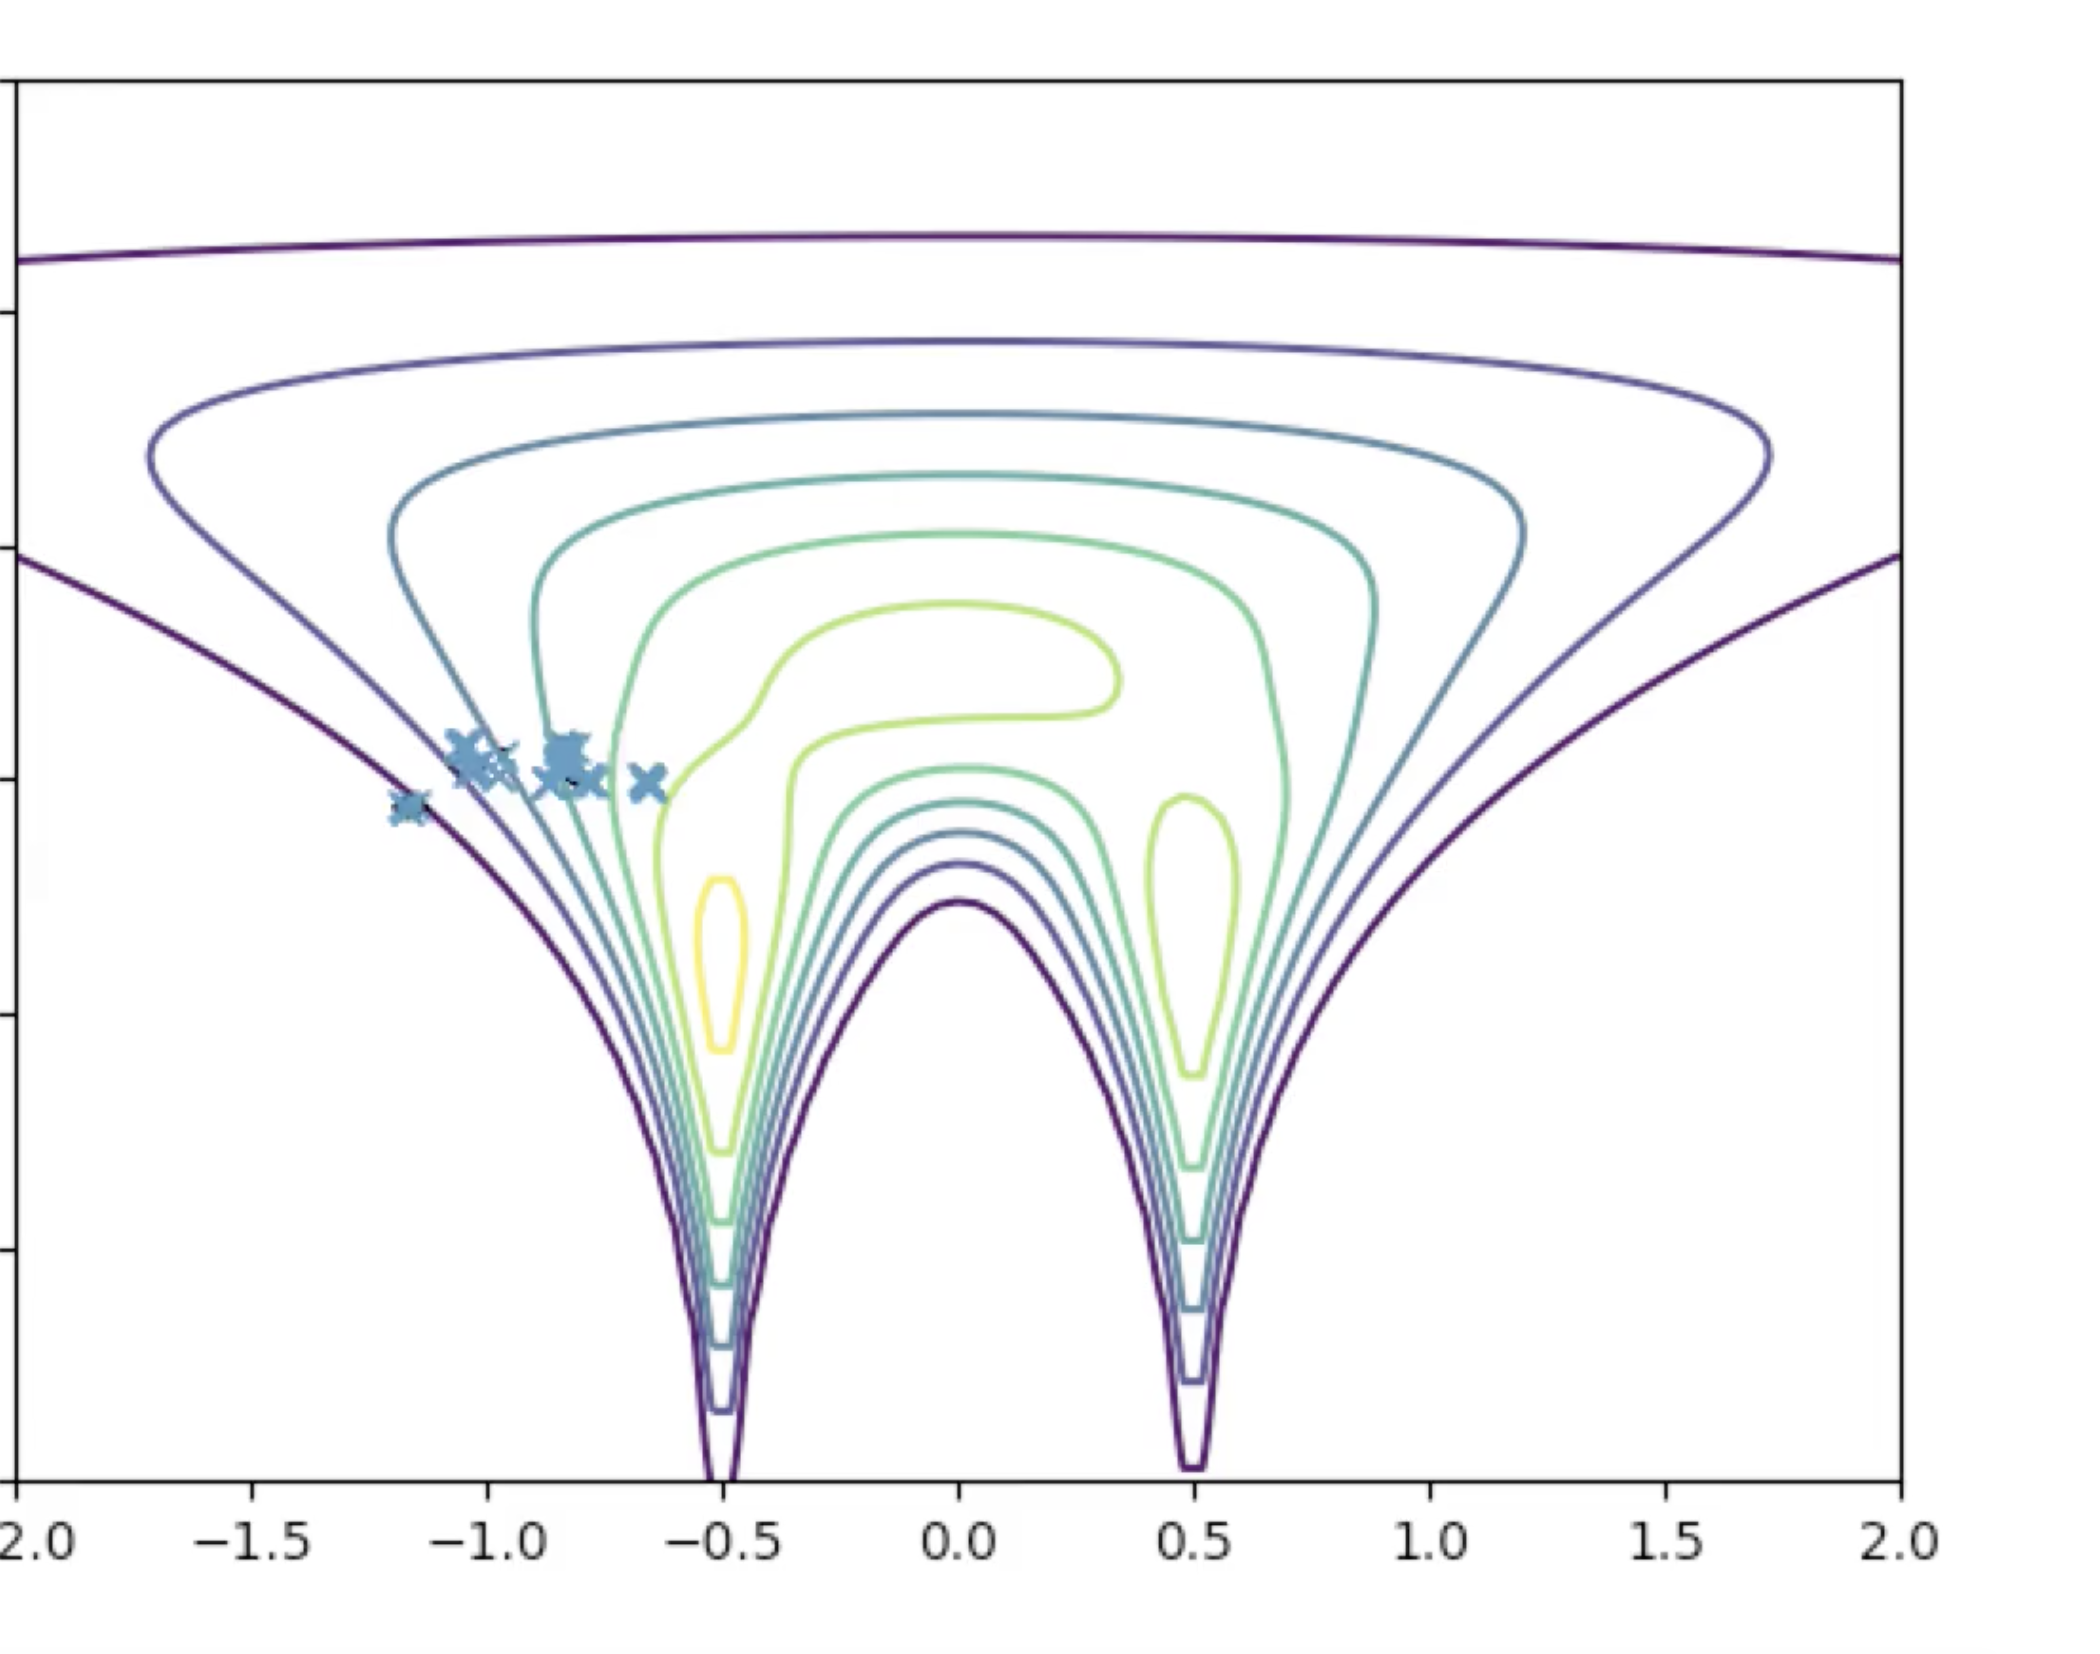
\includegraphics[width=.7\textwidth]{images/intro_animation_1.png}\\
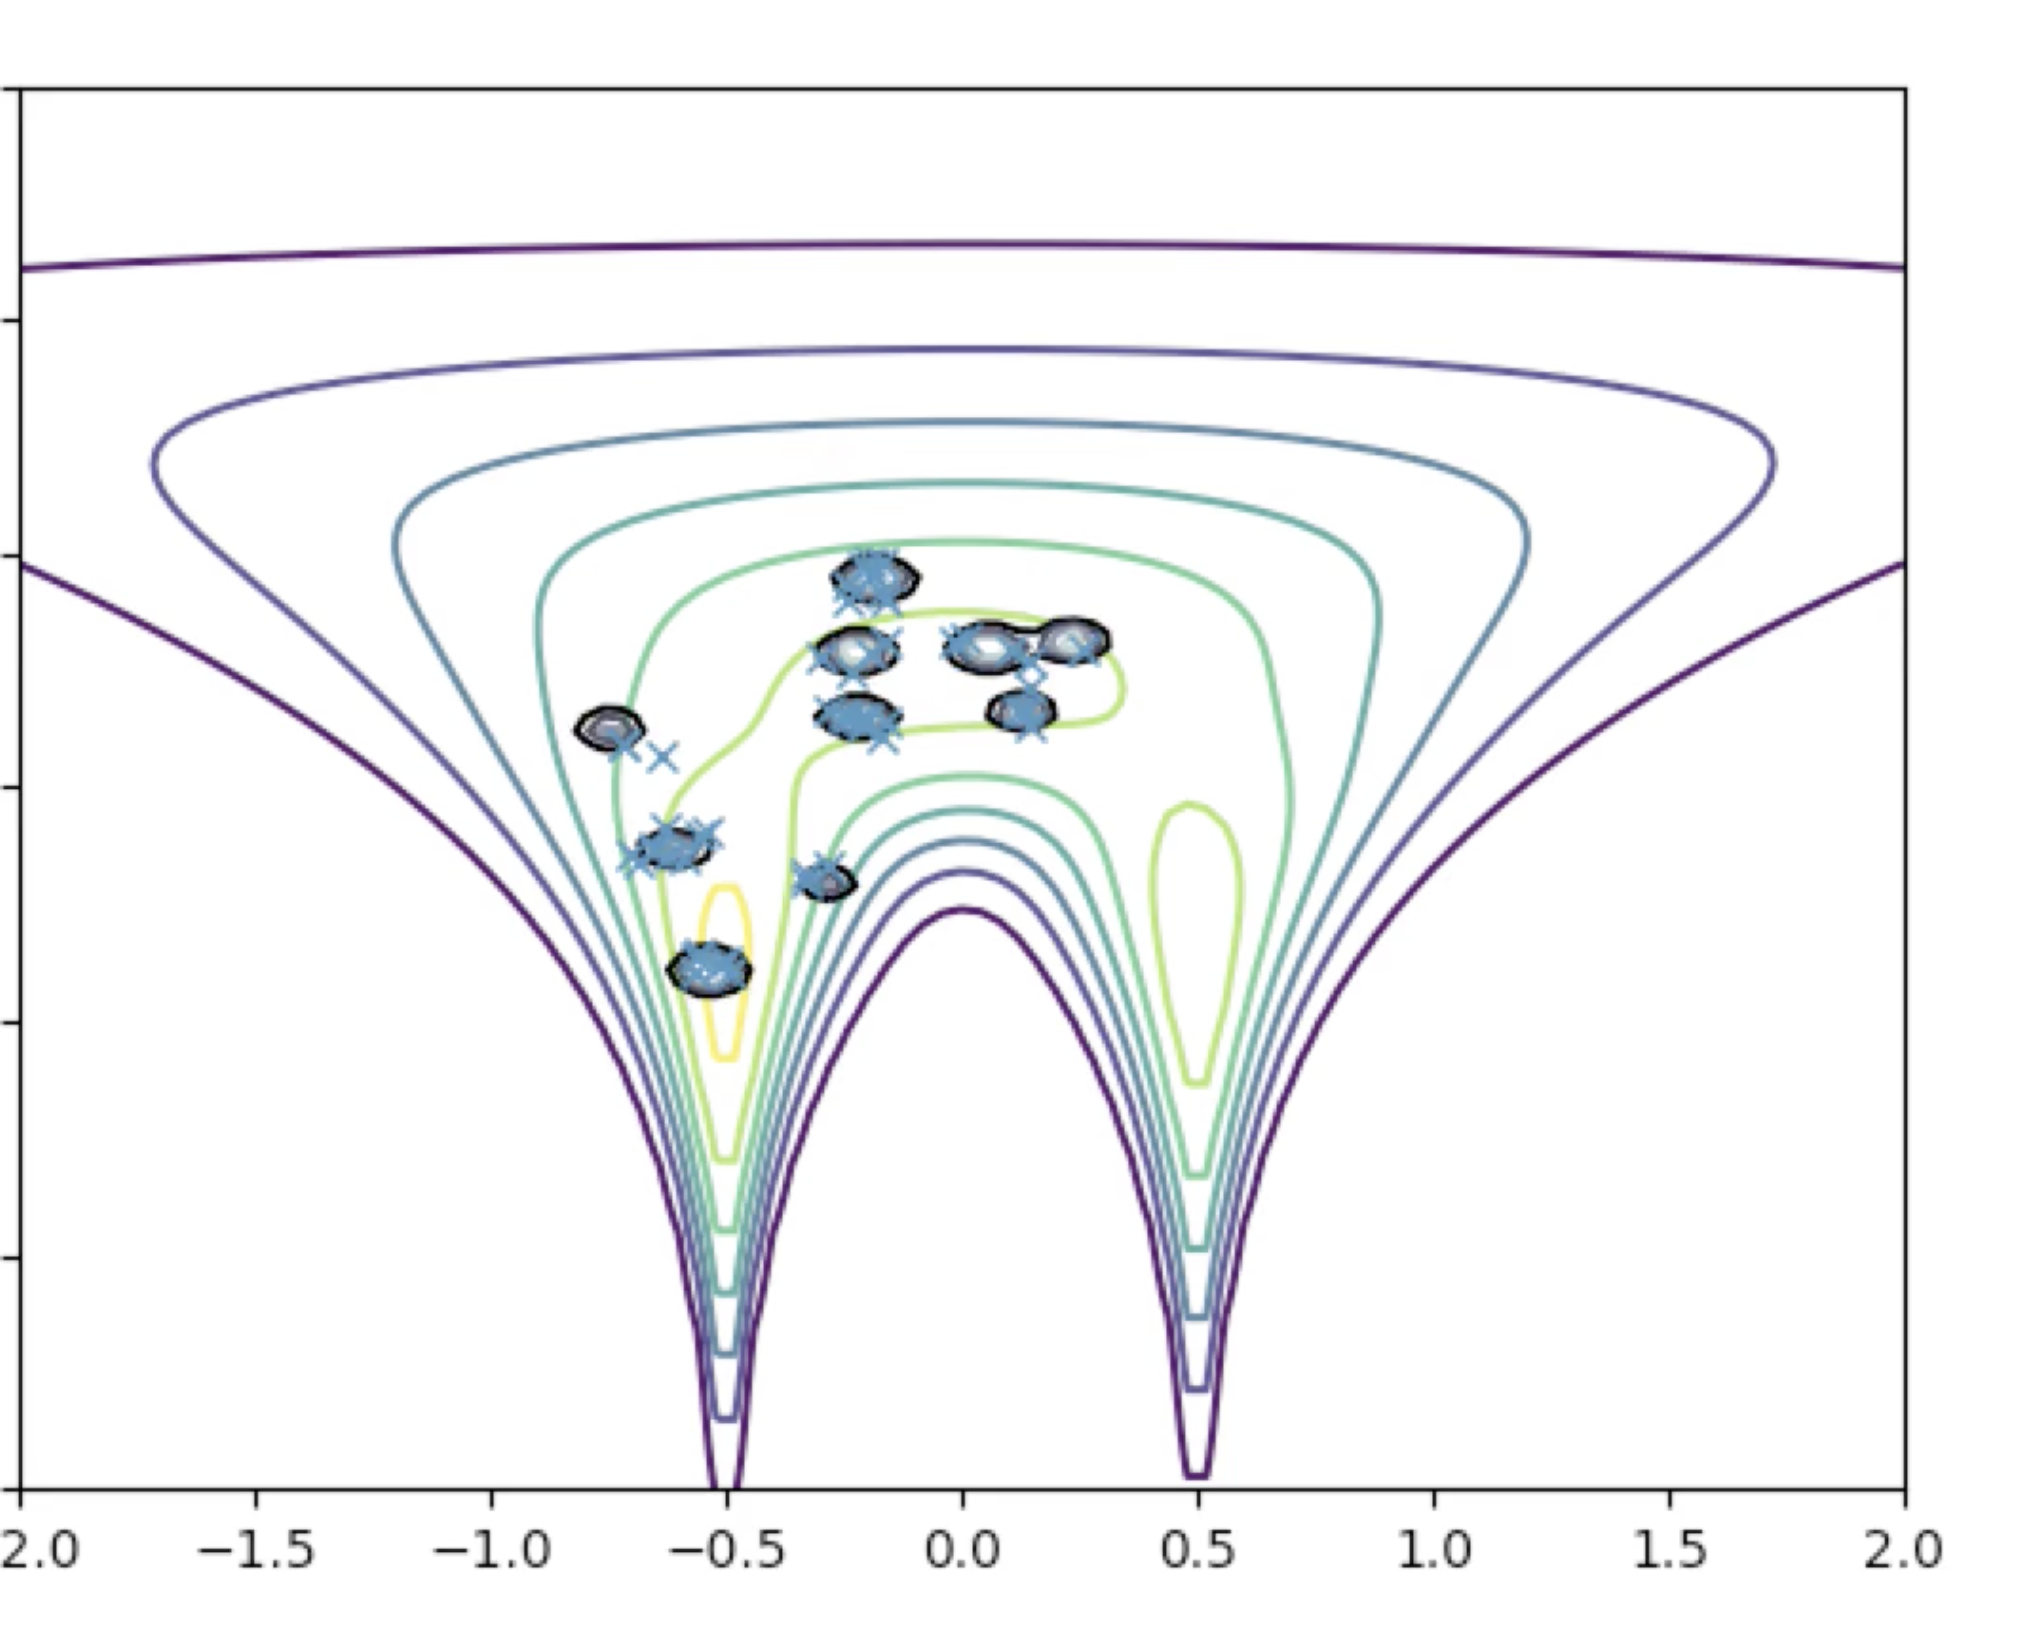
\includegraphics[width=.7\textwidth]{images/intro_animation_2.png}
\column{.5\textwidth}
\centering
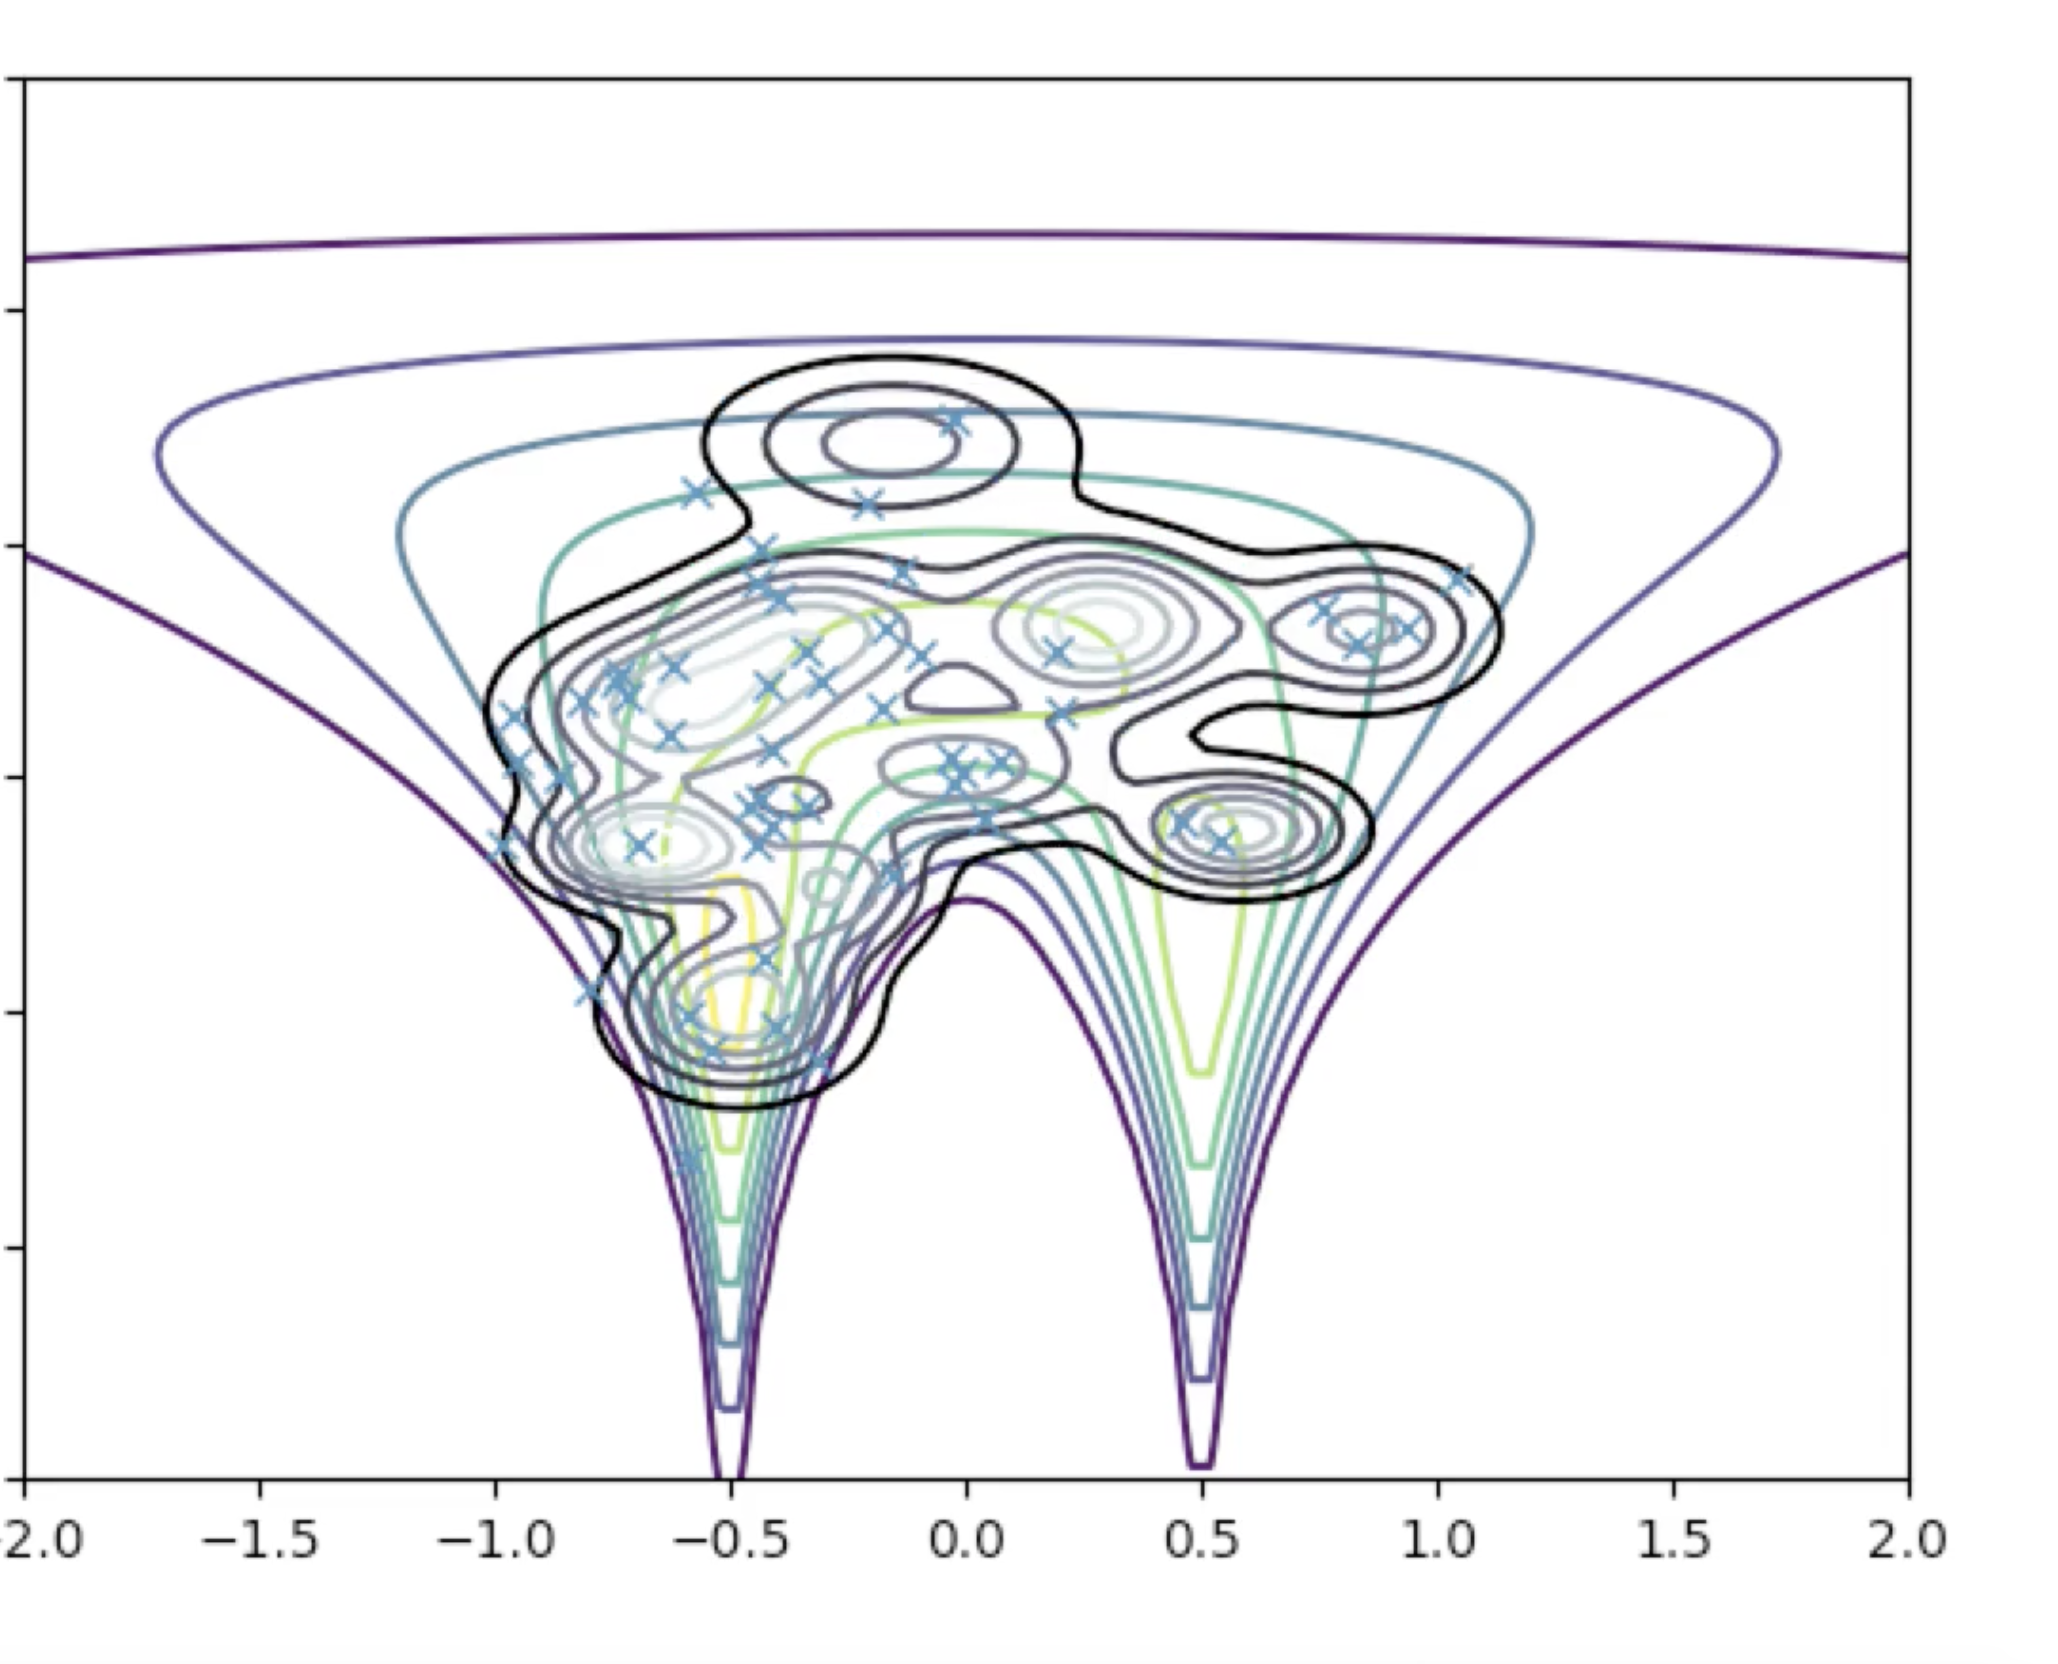
\includegraphics[width=.7\textwidth]{images/intro_animation_3.png}\\
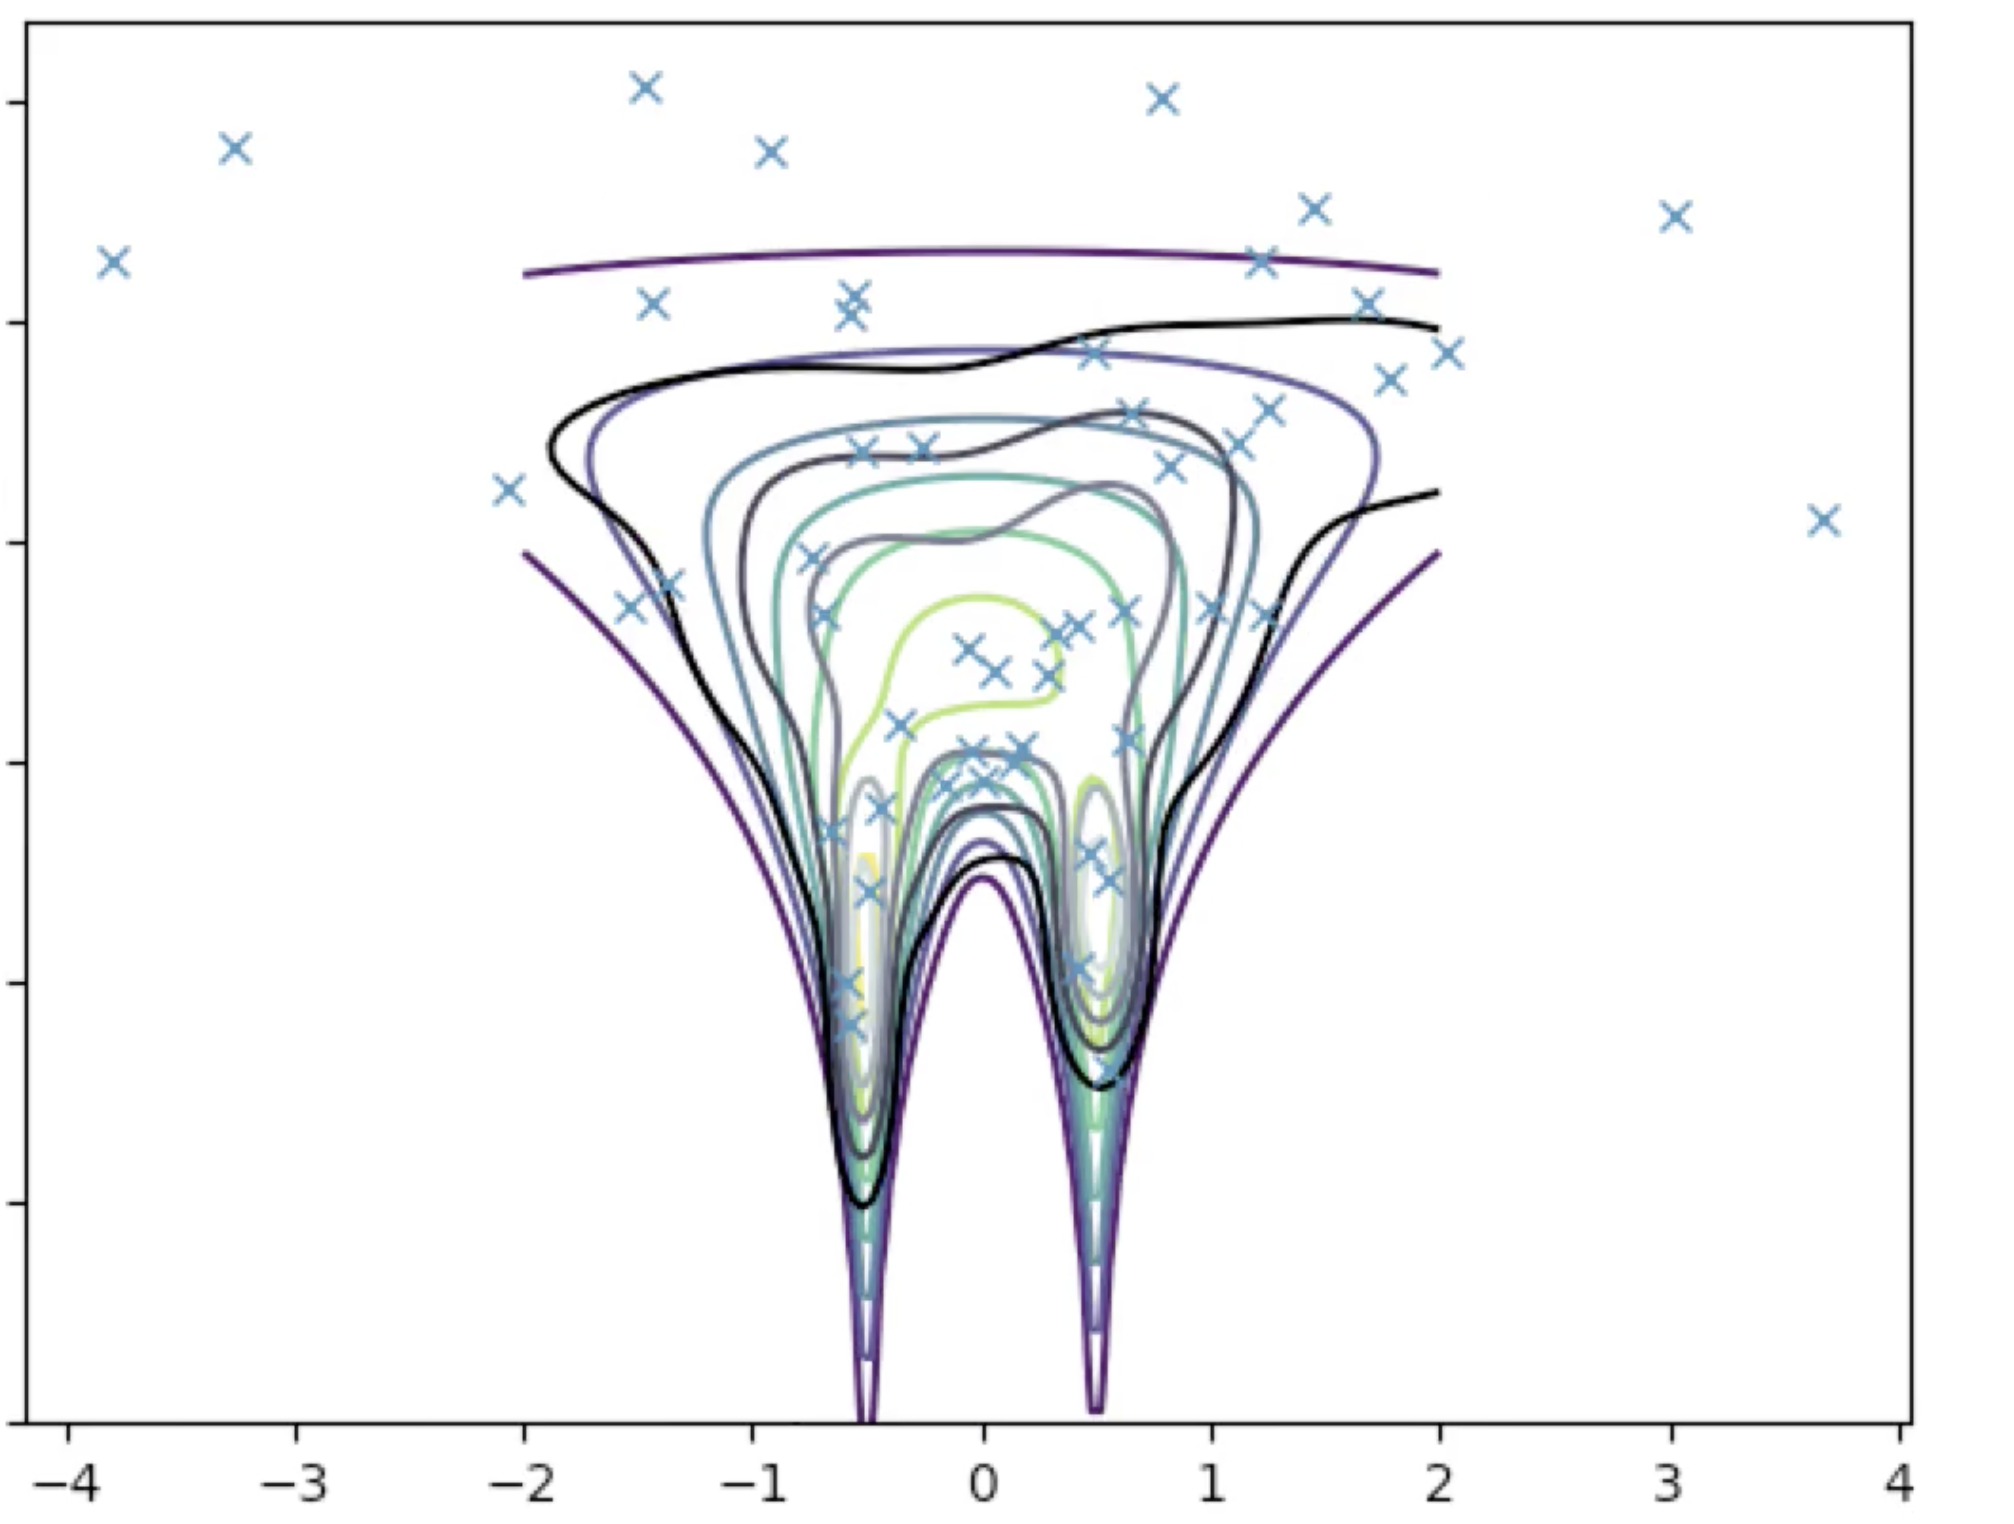
\includegraphics[width=.7\textwidth]{images/intro_animation_4.png}
\end{columns}

\vfill

\tiny Ranganath, R., Gerrish, S., \& Blei, D. (2014, April). Black box variational inference. In Artificial Intelligence and Statistics (pp. 814-822).
  \end{minipage}
  
\end{frame}


\subsection{Decompositions: Intuition on the cost function}
%%%%%%%%%%%%%%%%%%%%%%%%%%%%%%%%%%%%%%%%%%%%%%%%%%%
\begin{frame}{Decompositions of the VLBO}
\metroset{block=fill}
\begin{block}{Energy/Entropy Decomposition of the VLBO}
By simply appealing to properties of the logarithm and the definition of expectation, we obtain 
\begin{align*}
\VLBO(q) & = \ds\int  q(\+u) \; \ln p(\+x,\+u  \cond \+c) \wrt{\+u}   - \ds\int  q(\+u) \; \ln q(\+u) \wrt{\+u}  \\
& =  \underset{energy}{ \E_q \big[ \log p(\+x, \+u  \cond \+c ) \big] } + \underset{entropy}{ \mathbb{H} \big[q(\+u) \big] }  
\end{align*}

%Energy: It tries to place high probability on unobserved variables that are jointly likely with the data from the perspective of the model 
%Entropy: a regularizer; keeps the result from being a point mass (o/w var density would e.g. put all the prob mass on the most likely latent state for each data point) ; tries to maximize uncertainty. 
\end{block} 
\vfill \tiny \textbf{Q}  What is the effect of the entropy term?
\end{frame}


%%%%%%%%%%%%%%%%%%%%%%%%%%%%%%%%%%%%%%%%%%%%%%%%%%%
\begin{frame}{Decompositions of the VLBO}
\metroset{block=fill}
\begin{block}{Likelihood/Prior Decomposition of the VLBO}
By applying the chain rule to the preceding, and then reapplying the definition of KL divergence, we obtain another nice form

 \begin{align*}
\VLBO(q) &=   \E_q \big[ \log p(\+x, \+u \cond \+c) \big]  +  \mathbb{H} \big[q(\+u) \big] \\
& =  \E_q \big[ \log p(\+x, \+u \cond \+c) \big] - \E_q \big[ \log q(\+u) \big] \\
& =  \E_q \big[ \log p(\+x \cond \+u, \+c) \big] + \E_q \big[ \log p(\+u \cond \+c) \big] - \E_q \big[ \log q(\+u) \big] \\
&= \underset{expected \; log \; likelihood}{\E_q \big[ \log p(\+x \cond \+u, \+c) \big]}  -  \underset{divergence \; from \; prior}{\texttt{KL} \big(q(\+u ) \; || \; p(\+u \cond \+c)\big)}
\end{align*}
\end{block} 

 
%The first term is a negative reconstruction error; the second acts as a regularizer.  

Note that the first term grows in magnitude as the number of samples increases; thus, the prior's influence diminishes asymptotically.

\end{frame}

\subsection{The posterior perspective}
%%%%%%%%%%%%%%%%%%%%%%%%%%%%%%%%%%%%%%%%%%%%%%%%%%%
\begin{frame}{Maximizing the \VLBO minimizes the KL divergence \tiny (to the posterior)}  

%The variational density $q \in \mathcal{Q}$  which maximizes the \VLBO also minimizes the KL divergence from the target posterior $p(\+u \cond \+x, \+c)$ %to the variational density. 

By definition, the \texttt{KL} divergence from the target posterior to the variational density is given by
\begin{equation*}
\texttt{KL} (q(\+u) \; || \; p(\+u \cond \+x, \+c)) =  \E_q \bigg[\log \df{q(\+u )}{p(\+u \cond \+x, \+c)} \bigg] 
\end{equation*}

 

%\begin{equation*}
% \texttt{KL} (q(\+u) \; || \; p(\+u \cond \+x, \+c)) =  \E_q[\log q(\+u )]  - \E_q[ \log p(\+u \cond \+x, \+c)] 
%\end{equation*}

By the chain rule, we get 
\begin{align*} 
 \texttt{KL} (q(\+u) \; || \; p(\+u \cond \+x, \+c)) & = \explaintermbrace{energy/entropy decomposition}{ \E_q[\log q(\+u )]  - \E_q[ \log p(\+x,\+u \cond \+c)]} &&+\log p(\+x \cond \+c) \\
 & = \hphantom{blah} -\VLBO(q)  && +  \text{constant} 
 \end{align*}
 
%Note that the term $p(\+x \cond \+c)$, is constant in the minimization.  Thus, we may equivalently maximize the negative of the first two terms, which is the \VLBO.

 
\vfill \tiny \bf{Discuss:} What is the optimal variational density?

\end{frame}


%%%%%%%%%%%%%%%%%%%%%%%%%%%%%%%%%%%%%%%%%%%%%%%%%%%
\begin{frame}{Maximizing the \VLBO minimizes the KL divergence \tiny (to the posterior)}  

%The variational density $q \in \mathcal{Q}$  which maximizes the \VLBO also minimizes the KL divergence from the target posterior $p(\+u \cond \+x, \+c)$ %to the variational density. 

By definition, the \texttt{KL} divergence from the target posterior to the variational density is given by
\begin{equation*}
\texttt{KL} (q(\+u) \; || \; p(\+u \cond \+x, \+c)) =  \E_q \bigg[\log \df{q(\+u )}{p(\+u \cond \+x, \+c)} \bigg] 
\end{equation*}

 

%\begin{equation*}
% \texttt{KL} (q(\+u) \; || \; p(\+u \cond \+x, \+c)) =  \E_q[\log q(\+u )]  - \E_q[ \log p(\+u \cond \+x, \+c)] 
%\end{equation*}

By the chain rule, we get 
\begin{align*} 
 \texttt{KL} (q(\+u) \; || \; p(\+u \cond \+x, \+c)) & = \explaintermbrace{energy/entropy decomposition}{ \E_q[\log q(\+u )]  - \E_q[ \log p(\+x,\+u \cond \+c)]} &&+\log p(\+x \cond \+c) \\
 & = \hphantom{blah} -\VLBO(q)  && +  \text{constant} 
 \end{align*}
 
%Note that the term $p(\+x \cond \+c)$, is constant in the minimization.  Thus, we may equivalently maximize the negative of the first two terms, which is the \VLBO.

\metroset{block=fill}
\begin{block}{The optimal variational density}
The optimal variational density, $q^*(\+u)$ is the target posterior density $p(\+u \cond \+x, \+c)$ when the underlying variational family $\Q$ is unrestricted  
\end{block}

\end{frame}






%%%%%%%%%%%%%%%%%%%%%%%%%%%%%%%%%%%%%%%%%%%%%%%%%%%%
%\begin{frame}{How does VI accommodate the goal of
%statistical inference?}
%
%The optimal variational density, $q*$ can be related to  
%
%\begin{itemize}
%\item the \alert{target marginal}, $p(\+x \cond \+c)$.
%\item the \alert{target posterior}, 
%$p(\+u \cond \+x, \+c)$.
%\end{itemize}
%
%\end{frame}














%
%%%%%%%%%%%%%%%%%%%%%%%%%%%%%%%%%%%%%%%%%%%%%%%%%%%%
%\begin{frame}{Towards the target posterior perspective}
%
%\textbf{Remark} Since we generally can't compute the exact posterior, we are often in the situation of the second result, where we place constraints on $\Q$ and get the best possible approximation. 
%
%\end{frame}

\subsection{Summary}

%%%%%%%%%%%%%%%%%%%%%%%%%%%%%%%%%%%%%%%%%%%%%%%%%%%
\begin{frame}{Summary}

\begin{itemize}
\item VI is a general tool.  It is useful whenever you face intractable marginals.
%\item It's thus a general tool for modeling conditional probabilities 
\end{itemize}

\scriptsize
\begin{table}[ht]
%\caption{Key ingredients for VI in various modeling paradigms} % title of Table
\centering % used for centering table
\begin{tabular}{l | l l l l} % centered columns 
%heading
%\hline \\ [.5ex] % inserts single horizontal line
Model & Inferential & Intractable  &  Variational  & Posterior \\
& goal & marginal & density &  \\   [.8ex]
%& & & & (or ``posterior")\\
\hline \\ [.8ex] % inserts single horizontal line
General case & \text{infer about} $\+\theta$ & $p(\+x \cond \+c)$& $q(\+u)$ & $p(\+u \cond \+x, \+c)$  \\ [.8ex]
\hline \\ [.8ex] % inserts single horizontal line
Frequentist  & $\argmax_{\+\theta} \alert{p(\+x \cond \+\theta)}$  & \alert{$p(\+x \cond \+\theta)$} = $\ds\int p(\+x, \+z \cond \+\theta) \wrt{\+z}$  & $q(\+z)$ & \blue{$p(\+z \cond \+x, \+\theta)$}  \\
latent & & & & \\ [.8ex]
Bayesian  & $\alert{p(\+\theta \cond \+x)}$ & $ \blue{p(\+x)} = \ds\int p(\+\theta,\+x) \wrt{\+\theta}$ & $q(\+\theta)$ &  \alert{$p(\+\theta \cond \+x)$} \\ 
(non-latent) & & & & \\  [.8ex]
Bayesian  & $\alert{p(\+z, \+\theta \cond \+x)}$ &  $\blue{p(\+x)} = \ds\int p(\+\theta,\+x, \+z) \wrt{\+\theta} \wrt{\+z}$  &  $q(\+z, \+\theta)$ & \alert{$p(\+z, \+\theta \cond \+x)$} \\
latent & & & & \\  [.8ex]
\end{tabular}
\label{vi_table} % is used to refer this table in the text
\end{table}
 
\end{frame}

%%%%%%%%%%%%%%%%%%%%%%%%%%
\begin{frame}{How does VI accommodate the goal of statistical inference?}

Given selection of variational family $\Q$, the optimal variational density $q^*$ ...

\metroset{block=fill}
\begin{block}{The marginal perspective}

\begin{itemize}

%We can now maximize an objective function which is as similar as possible to the true objective, the marginal likelihood $p(\+x \cond \+\theta)$. %(So it would seem to provide a "good" estimate of $\+\theta$.) 
% Shorter: We can now find $\+\theta$ which maximizes a quantity approximating the marginal likelihood. 
% Finding parameter $\widehat{\+\theta}_{\text{VI}}$ maximizing  $\VLBO(q^*)$ amounts to maximizing an objective function which is as similar as possible to the true objective, the marginal likelihood $p(\+x \cond \+\theta)$

\item \textit{For frequentist models}: ... makes the \VLBO best approximate the  \alert{target marginal likelihood, $p(\+x \cond \+\theta)$}, which is what we wanted to maximize.
\item \textit{For Bayesian models}: ... raises the (approximate) evidence term $\blue{p(\+x)}$ (the term used for Bayesian model comparison) as high as possible. %(So it would seem to provide a "good" distribution over $\+u$.) 
\end{itemize}

\end{block} 


\metroset{block=fill}
\begin{block}{The posterior perspective}

\begin{itemize}
\item \textit{For Bayesian models}:  ...  is the family member which is closest to the\alert{ target  posterior $p(\+u \cond \+x)$}.
\item \textit{For frequentist models}: ... provides the best substitution $q^*(\+z) \approx \blue{p(\+z\cond \+x, \+\theta^{\text{curr}})}$ into the E-step of the EM algorithm\footnote{See next section for more information.}
\end{itemize}

\end{block} 
\end{frame}


\subsection{Evaluation (in context)}


%%%%%%%%%%%%%%%%%%%%%%%%%%%%%%%%%%%%%%%%%%%%%%%%%%
\begin{frame}{Approximate Bayesian Inference}

\begin{itemize}
\item The two most prominent strategies for approximating intractable posteriors are VI and Markov Chain Monte Carlo (MCMC). 
\item MCMC  uses \alert{sampling}.  We construct a Markov chain over model parameters.  The stationary distribution is the posterior.  We approximate the posterior with samples.
\item VI uses \alert{approximation}.  A tractable approximating family is chosen, and parameters are optimized to be close to the posterior.
\end{itemize}

\end{frame}

\begin{frame}{Variational Inference vs MCMC}

Variational Inference scales better to large datasets.

\begin{figure}
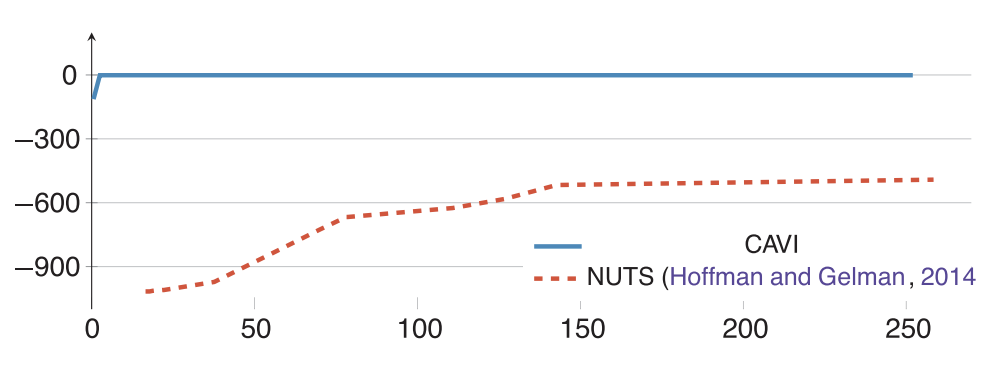
\includegraphics[width=\textwidth]{images/CAVI_vs_HamiltonianMCMC}
\caption{ Comparison of CAVI to a Hamiltonian Monte Carlo-based sampling technique.  The plot shows log predictive test set accuracy by training time (minutes).  CAVI fits a Gaussian mixture model to 10,000 images in less than a minute.}
\end{figure}
\vfill
\tiny Blei, D. M., Kucukelbir, A., \& McAuliffe, J. D. (2017). Variational inference: A review for statisticians. Journal of the American statistical Association, 112(518), 859-877.
\end{frame}


\begin{frame}{Variational Inference vs. Expectation Propagation}
\footnotesize
Let us fix a distribution $P$ and consider two optimization strategies
\metroset{block=fill}
\begin{block}{Variational Inference}
\begin{minipage}{.3\textwidth}
Minimizing \\
$\texttt{KL}(\blue{Q} || \red{P})$ \\
\tiny $ = \E_Q \bb{\log \frac{q(x)}{p(x)}}$
\end{minipage}
\hfill
\begin{minipage}{.6\textwidth}
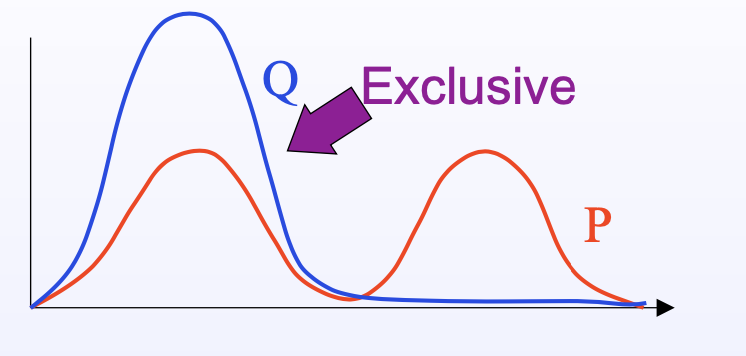
\includegraphics[width=.9\textwidth]{images/kl_for_vi}
\end{minipage}
\end{block}

\metroset{block=fill}
\begin{block}{Expectation Propagation}
\begin{minipage}{.3\textwidth}
Minimizing \\
$\texttt{KL}(\red{P} || \blue{Q})$ \\
\tiny $ = \E_P \bb{\log \frac{p(x)}{q(x)}}$
\end{minipage}
\hfill
\begin{minipage}{.6\textwidth}
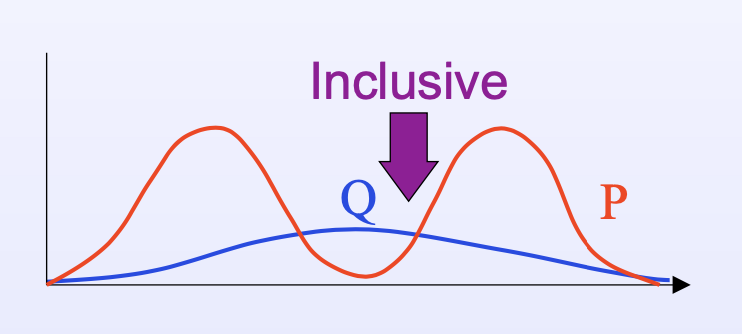
\includegraphics[width=.9\textwidth]{images/kl_for_ep}
\end{minipage}
\end{block}
\hfill \tiny Image Credit: Tushar Tank \\
\vfill \tiny \bf{Q:}  What does this say about VI?  Which one would you prefer to use?    
\end{frame}

%%%%%%%%%%%%%%%%%%%%%%%%%%%%%%%%%%%%%%%%%%%%%%%%%%
\begin{frame}{Shortcoming: VI underestimates variance of the true posterior}


	\begin{figure}
	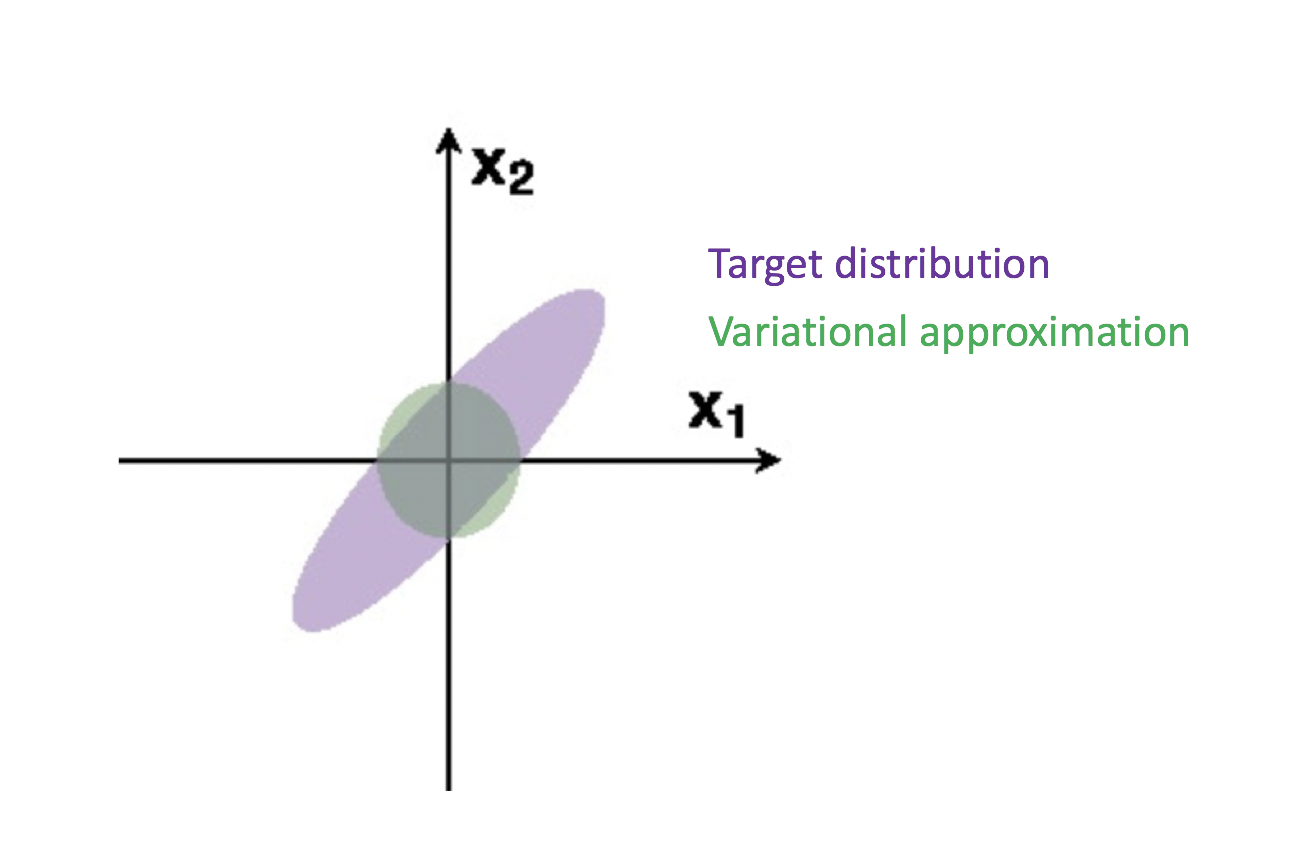
\includegraphics[width=.7\textwidth]{images/underfit_variance_2.png}
	\end{figure}


\[ \texttt{KL} (q(\+u) \; || \; p(\+u \cond \+x, \+c)) =  \E_q \bigg[\log \df{q(\+u )}{p(\+u \cond \+x, \+c)} \bigg]  \]
 
Intuition 
\begin{itemize}

\item If $ \green{q(\+u )}$ is low, then we don't care (because of the expectation).   
\item If $ \green{q(\+u )}$ is high and $ \purple{p(\+x,\+u \cond \+c)}$  is low, then we pay a price
%\item If $ \green{q(\+u )}$ is high and $\purple{p(\+x,\+u \cond \+c)}$  is high, then we are happy  
\end{itemize}

\end{frame}


%%%%%%%%%%%%%%%%%%%%%%%%%%%%%%%%%%%%%%%%%%%%%%%%%%
\begin{frame}{Modern application}

  \begin{minipage}[t][.9\textheight]{\textwidth}

We can compose probabilistic graphical models with neural networks to exploit their complementary strengths.  

\vspace{.2in}

\centering
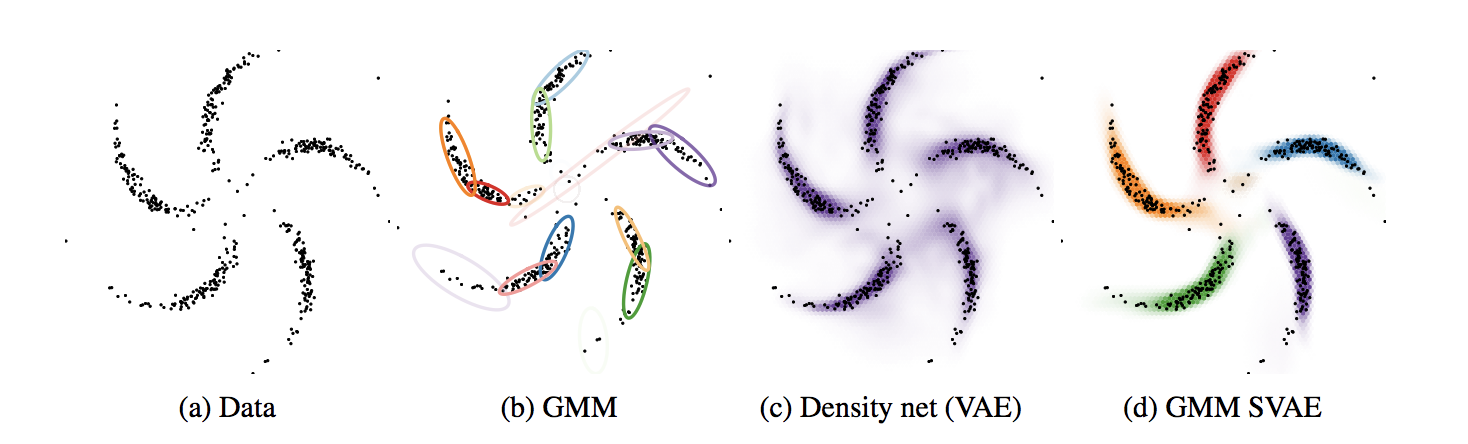
\includegraphics[width=.95\textwidth]{images/composing_pgms_with_nns}

\vspace{.2in}

The resulting model is expressive, but also interpretable/decomposable.\\

    \vfill

\tiny Johnson, M., Duvenaud, D. K., Wiltschko, A., Adams, R. P., \& Datta, S. R. (2016). Composing graphical models with neural networks for structured representations and fast inference. In Advances in neural information processing systems (pp. 2946-2954).

  \end{minipage}
  
\end{frame}




%%%%%%%%%%%%%%%%%%%%%%%%%%%%%%%%%%%%%%%%%%%%%%%%%%
\section{Variational Inference and Expectation Maximization}




\begin{frame}{Expectation Maximization (EM)}

The EM algorithm refines an initial guess $\+\theta^{(0)}$ via the recursion
\[ \+\theta^{(t+1)} =  \text{argmax}_{\+\theta} \; \E_{p(\+z \cond \+x , \+\theta^{(t)})} \bigg[ \ln p(\+x, \+z \cond \+\theta) \bigg] \]
until convergence to a local optimum.

\metroset{block=fill}
\begin{block}{Example: Gaussian Hidden Markov Model}

\textit{E-step}:  Compute $p_i := p(z_i \cond \+x_i, \+\theta^{(t)})$ via the forward-backward algorithm. 

\textit{M-step}: Just a computation of \alert{weighted} empirical means and variances:
\[ \widehat{\+\mu}_k^{(t)} = \df{\ds\sum_i \alert{(p_i = k)} \, \+x_i}{\ds\sum_i \alert{(p_i=k)}},  \quad \quad \widehat{\+\Sigma}_k^{(t)} = \df{\ds\sum_i \alert{(p_i = k)} \; (\+x_i-\widehat{\+\mu}^{(t)}) (\+x_i-\widehat{\+\mu}^{(t)})^T }{\ds\sum_i \alert{(p_i = k)}} \] 
\end{block}

\vfill \vfill

%\tiny Example in cybersecurity: Kantchelian, A., et al. (2015). \textit{Better malware ground truth: Techniques for weighting anti-virus vendor labels.} In Proceedings of the 8th ACM Workshop on Artificial Intelligence and Security (pp. 45-56). ACM.


\end{frame}


\justfor{long}{
	\begin{frame}{Expectation Maximization (EM)}
	
	The EM algorithm refines an initial guess $\+\theta^{(0)}$ via the recursion
	\[ \+\theta^{(t+1)} =  \text{argmax}_{\+\theta} \; \E_{p(\+z \cond \+x , \+\theta^{(t)})} \bigg[ \ln p(\+x, \+z \cond \+\theta) \bigg] \]
	until convergence to a local optimum.
	
	 
	
	\metroset{block=fill}
	\begin{block}{Example: Exponential Hidden Markov Model}
	
	\textit{E-step}:  Compute $p_i := p(z_i \cond x_i, \+\theta^{(t)})$ via the forward-backward algorithm. 
	
	\textit{M-step}: Just a computation of \alert{weighted} empirical reciprocal means:
	\[ \widehat{\+\theta}_k^{(t)} = \df{\ds\sum_i \alert{(p_i = k)}}{  \ds\sum_i \alert{(p_i = k)} \, x_i} \]
	\end{block}
	
	\vfill \vfill
	
	\tiny Example in cybersecurity: Kantchelian, A., et al. (2015). \textit{Better malware ground truth: Techniques for weighting anti-virus vendor labels.} In Proceedings of the 8th ACM Workshop on Artificial Intelligence and Security (pp. 45-56). ACM.
	
	
	\end{frame}
}


%%%%%%%%%%%%%%%%%%%%%%%%%%%%%%%%%%%%%%%%%%%%%%%%%%%%%
%\begin{frame}{Towards the target posterior perspective}
%\metroset{block=fill}
%\begin{block}{The optimal unrestricted variational distribution}
%
%Here we show that the optimal variational distribution, $q^*(\+u)$ is the target posterior distribution $p(\+u \cond \+x, \+c)$ when the underlying variational family $\Q$ is unrestricted, i.e. can be any probability distribution.   
%
%
%Take ${q(\+u)} = p(\+u \cond \+x, \+c)$. Then we have
%\begin{align*}
% \VLBO(q) &= \ds\int p(\+u \cond \+x, \+c) \ln \bigg( \df{p(\+x, \+u \cond \+c)}{p(\+u \cond \+x, \+c)} \bigg)  \wrt{\+\theta} \\
%  &= \ds\int p(\+u \cond \+x, \+c) \ln p(\+x \cond \+c) \wrt{\+u} \\ 
%  &= \ln p(\+x \cond \+c) 
%\end{align*}
%
%In other word, the lower bound from is tight.  Thus, $ p(\+u \cond \+x, \+c)$ maximizes \VLBO(q).
%\end{block} 
%\end{frame}


\begin{frame}{EM from the perspective of VI}

 
%TOSAY:  What I want to do now is describe EM from the perspective of VI.  This will (1) give an alternate justification for the formula, but also (2) allow for generalization to the intractable cases.
 
For a frequentist latent variable model, the \VLBO is 

\begin{equation*} 
\VLBO(q_\+z, \theta) = \E_q \big[ \log p(\+x, \+z \cond \+\theta) \big]  +  \mathbb{H} \big[q(\+z) \big]  % \label{latent_var_elbo} 
\end{equation*}
%TOSAY: as always, what goes inside the expectation for the energy term is the joint between the data x and unobserved rv's u (of course conditioning on whatever is constant)

%via the \texttt{ELBO} of Equation \eqref{latent_var_elbo}. \cite{beal_diss} 

\pause 

Using coordinate ascent \tiny (in the sense of variational calculus) \normalsize ,  we get the following update equations: 

\begin{align}
\textbf{q update}: \quad & q_{\+z}^{(t+1)} = \text{argmax}_{q_\+z} \; \VLBO (q_\+z ; \+\theta^{(t)} ) \label{q_update} \\
\textbf{ $\+\theta$ update}: \quad & \+\theta^{(t+1)} = \text{argmax}_{\+\theta} \; \VLBO (q_{\+z}^{(t+1)} ; \+\theta )\label{theta_update} 
\end{align} 

\pause
 
As argued earlier, we can solve the \textit{q update} exactly by setting   
\[ q_{\+z}^{(t+1)} =   p(\+z \cond \+x; \+\theta^{(t)})\]  
 
in which case the \textit{ $\+\theta$ update} becomes  \tiny (what?) \normalsize \pause 
\begin{equation}
 \+\theta^{(t+1)} =  \text{argmax}_{\+\theta} \; \E_{p(\+z \cond \+x , \+\theta^{(t)})} \bigg[ \ln p(\+x, \+z \cond \+\theta) \bigg] \label{EM}
\end{equation}
 
which is precisely the EM algorithm. 

% In other words, the EM algorithm is a special case of variational inference where we can compute $p(\+z \cond \+x, \+\theta)$ and therefore utilize that as our optimal variational $q$.  

\end{frame}

%%%%%%%%%%%%%%%%%%%%%%%%%%
\begin{frame}{EM as coordinate ascent on the \VLBO }

	\begin{figure}
	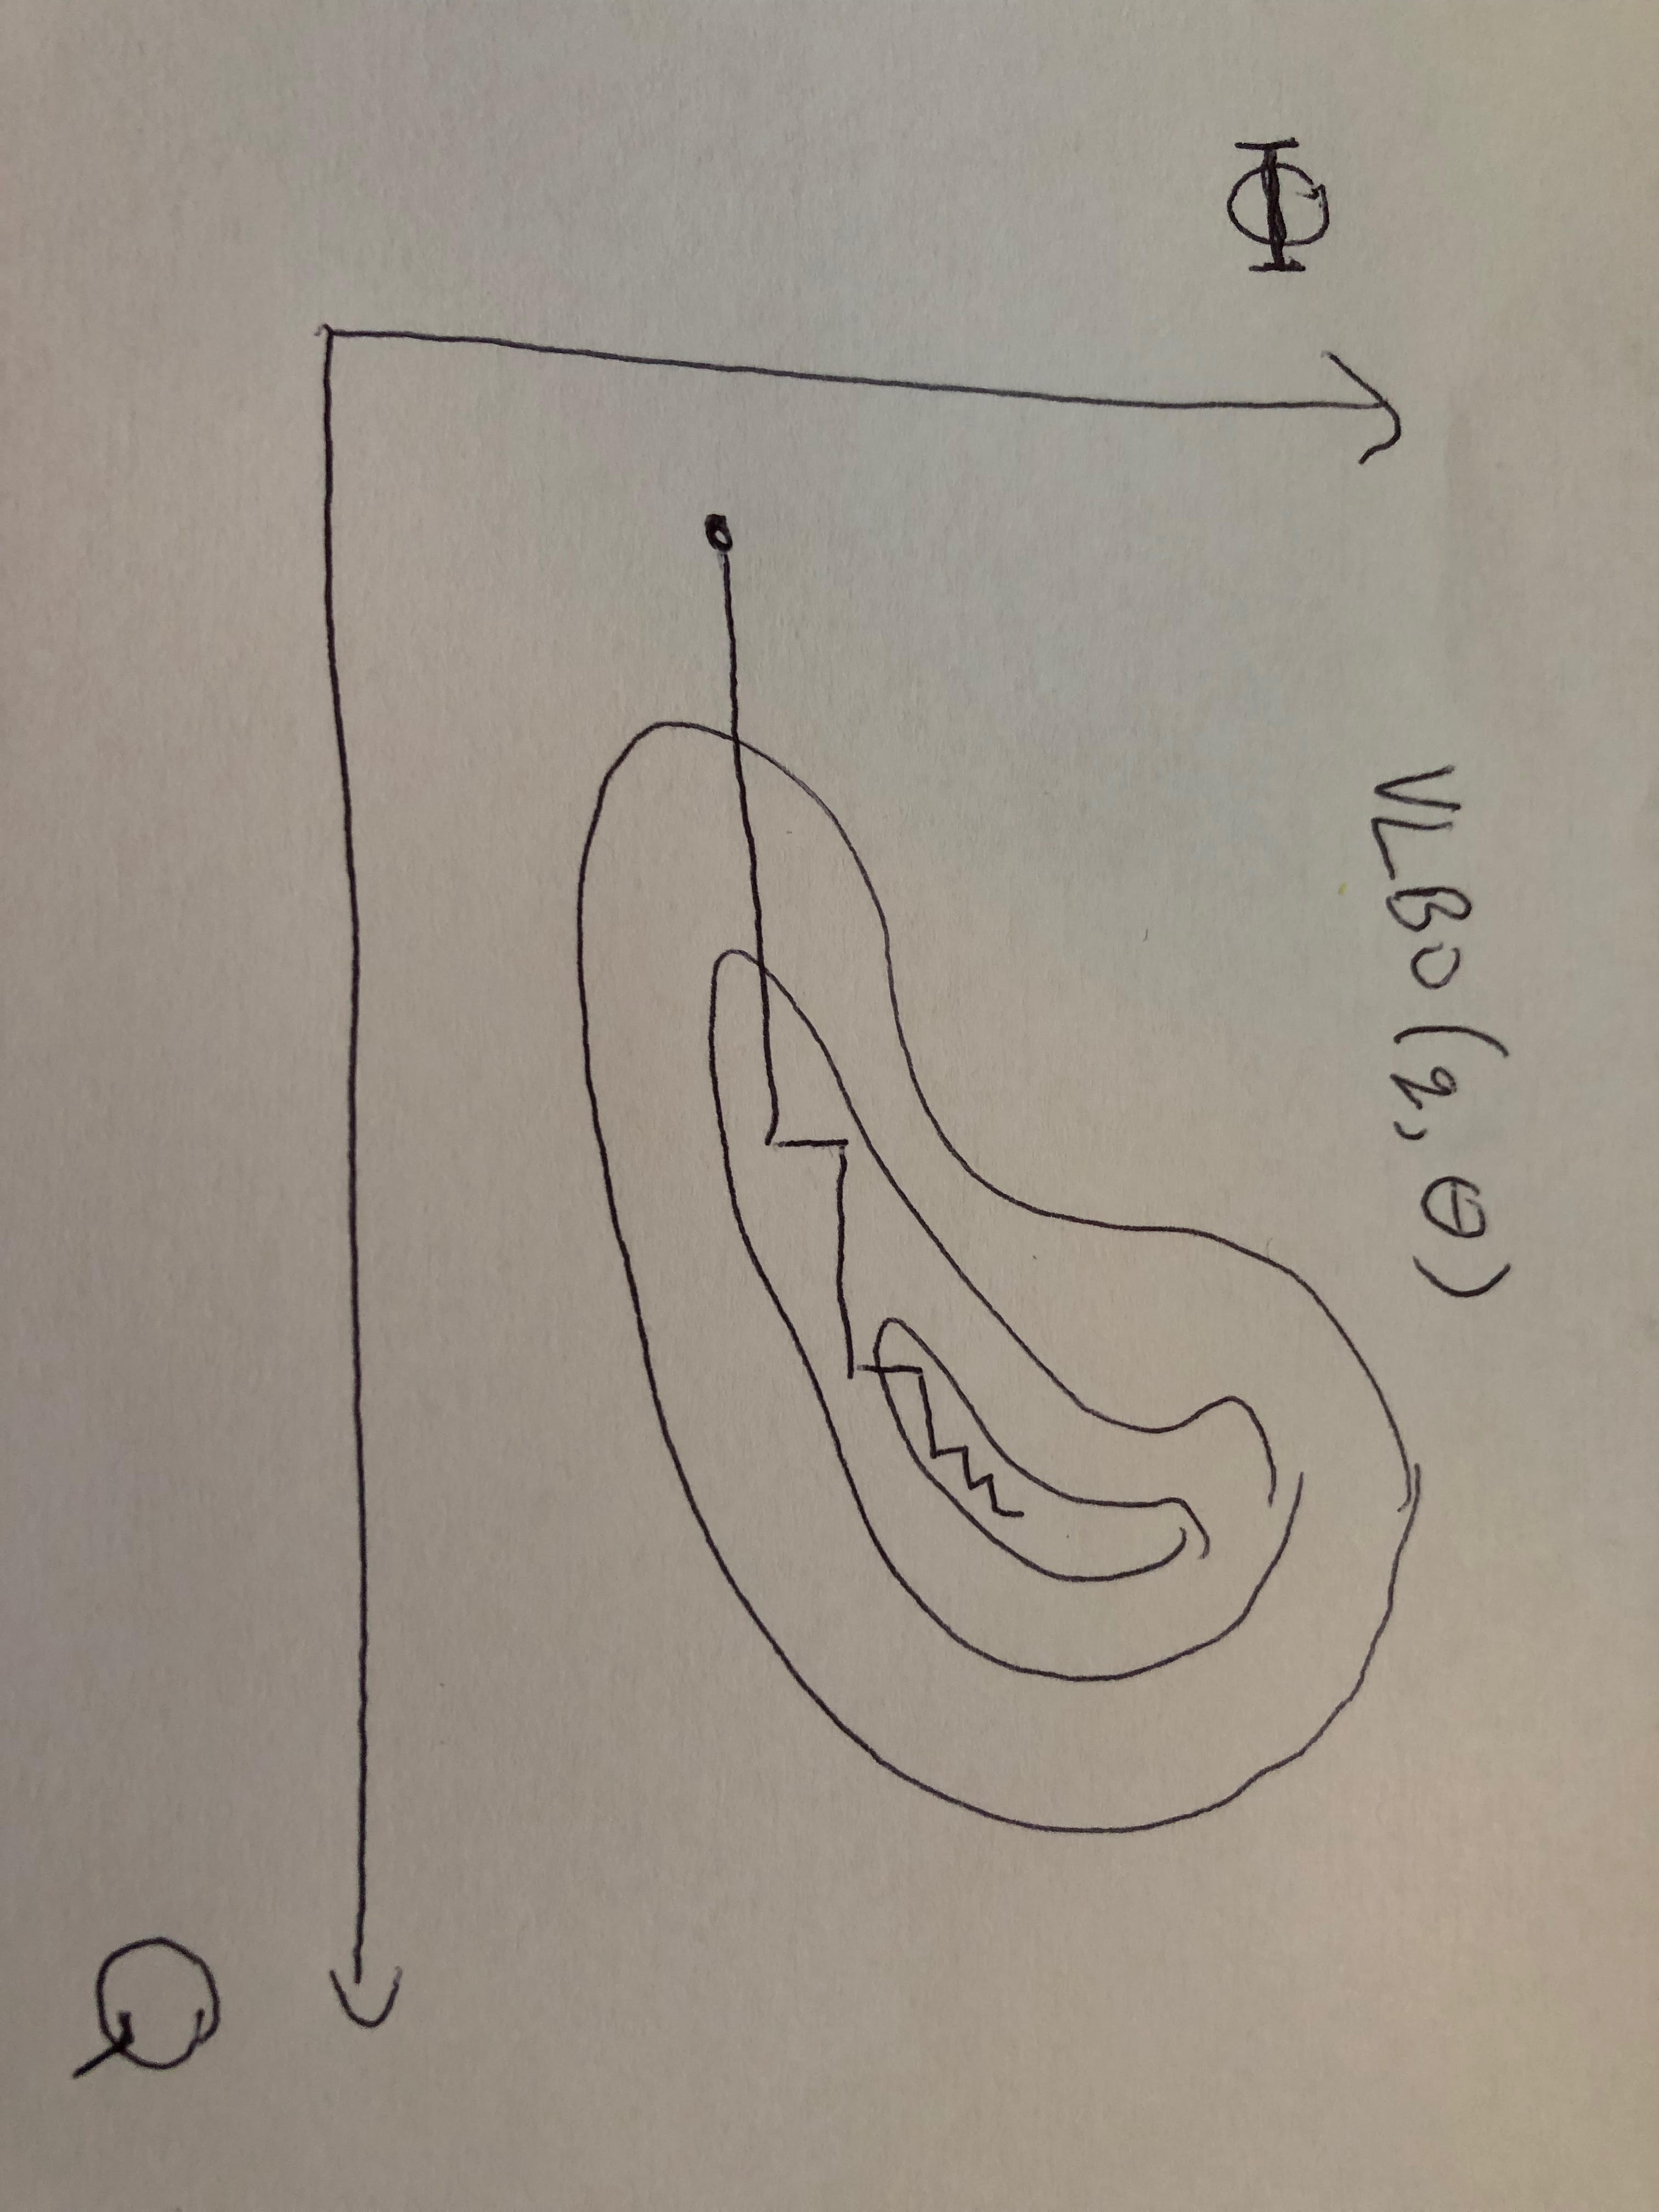
\includegraphics[width=.55\textwidth, angle=90]{images/em_is_perfect_vi.jpg}
	\end{figure}

 
\begin{itemize}
\item If $\Q$ unrestricted, we have EM   
\item What if we restrict $\Q$ ?
%TO SAY: need to for: LDA, BHMM, VAE, BBVI, ADVI,....
\end{itemize}

\end{frame}


%%%%%%%%%%%%%%%%%%%%%%%%%%
\begin{frame}{Variational Expectation Maximization (VEM)}

Consider a \alert{frequentist latent variable model}. Since we don't always have access to $p(\+z \cond \+x, \+\theta)$, we may restrict our variational family $\Q$ to some convenient form.  In this case, 
coordinate ascent on the \VLBO is given by:

\begin{align*}
q_{\+z}^{(t+1)} &= \text{argmax}_{q_\+z \in \mathcal{Q}} \; \VLBO  (q_\+z ; \+\theta^{(t)} )\label{ve_update} \\ 
% & \stackrel{\text{(Sec 1.2)}}{=} \text{argmin}_{q_\+z \in \mathcal{Q}} \; \KL{q_\+z}{p(\+x \cond \+y, \+\theta^{(t)})} \label{ve_update} \\
\+\theta^{(t+1)} &= \text{argmax}_{\+\theta} \; \E_{q_{\+z}^{(t+1)}} \bigg[ \ln p(\+x, \+z \cond \+\theta) \bigg]
\end{align*} 

which generalizes the EM algorithm. %to situations where we cannot compute $p(\+z \cond \+x, \+\theta)$.
\end{frame}

\justfor{long}{%
\begin{frame}{Extension: Variational MAP}

Consider a \alert{Bayesian latent variable model}. Recall that a(n unscrupulous) Bayesian will sometimes compute a maximimum a posteriori (MAP) estimate of parameter $\+\theta$.  
\begin{equation}
\+\theta_{\text{MAP}}:=  \text{argmax}_{\+\theta} \; p (\+x , \+\theta) = \text{argmax}_{\+\theta} \ds\int p(\+x,\+z , \+\theta) \wrt{\+z} 
\label{map_latent_vars}
\end{equation} To obtain $\+\theta_{\text{MAP}}$ here, we swap $p(\+x,\+z, \+\theta)$ for $p(\+x,\+z \cond \+\theta)$ in the \VLBO and then immediately obtain the same algorithm but with altered M-step 

\begin{align*}
q_{\+z}^{(t+1)} &= \text{argmax}_{q_\+z \in \mathcal{Q}} \; \VLBO  (q_\+z ; \+\theta^{(t)} )\label{ve_update} \\ 
% & \stackrel{\text{(Sec 1.2)}}{=} \text{argmin}_{q_\+z \in \mathcal{Q}} \; \KL{q_\+z}{p(\+x \cond \+y, \+\theta^{(t)})} \label{ve_update} \\
\+\theta^{(t+1)} &= \text{argmax}_{\+\theta} \; \E_{q_{\+z}^{(t+1)}} \bigg[ \ln p(\+x, \+z \cond \+\theta) \bigg] + \blue{\ln p(\+\theta)} 
\end{align*} 

\end{frame}
}


	\begin{frame}{Variational Bayes Expectation Maximization (VBEM)}
	
	Consider a \alert{Bayesian latent variable model}. % So again we marginalize over $p(\+x, \+z, \+\theta)$ instead of $p(\+x, \+z \cond \+\theta)$. But this time we want the full posterior.   
	So we need to swap $p(\+x,\+z, \+\theta)$ for $p(\+x,\+z \cond \+\theta)$ in the \VLBO.
	
	
	If we construct the variational density with the factorization  
	\[  q(\+z,\+\theta)=q_\+z(\+z) q_{\+\theta}(\+\theta)\]
	
	
	then the \VLBO becomes
	
	\begin{equation}
	\VLBO (q_\+z(\+z), q_\+\theta(\+\theta)):=  \ds\int \ds\int  q_\+z(\+z) q_\+\theta(\+\theta) \; \ln \bigg( \df{p(\+z, \+\theta, \+x)}{q_\+z(\+z) q_\+\theta(\+\theta)} \bigg) \wrt{\+\theta} \wrt{\+z}  \label{VLBO_bayesian_latent}
	\end{equation}
	
	 
	We can perform coordinate ascent on the \VLBO with respect to the densities $q_\+z$ and $q_{\+\theta}$: 
	
	\begin{align*}
	\textbf{VB-E step}: \quad & q_{\+z}^{(t+1)} = \text{argmax}_{q_\+z} \; \VLBO (q_\+z \, ; \, q_{\+\theta}^{(t)} )  \\
	\textbf{VB-M step}: \quad & q_{\+\theta}^{(t+1)} = \text{argmax}_{q_{\+\theta}} \;  \VLBO (q_{\+z}^{(t+1)}  \, ; \, q_{\+\theta}) \\
	\end{align*} 
	
	\end{frame}
	
	\justfor{short}{
	\begin{frame}{VBEM: Derivation}
	\begin{center}
	See notes. 
	\end{center}
	\end{frame}
	}
	
	\justfor{long}{
	\begin{frame}{VBEM: Derivation}
	Because the VLBO is a functional, the update equations can be derived via variational calculus.  
	
	\textbf{Theorem} (Gelfand \& Foman)  Let $V[q]$ be a functional of the form 
\[ \ds\int_a^b F(u,q,q') dx \]
defined on the set of functions $q(u)$ which have continuous first derivatives in $[a,b]$ and satisfy the boundary conditions $q(a)=A, q(b)=B$. Then a necessary condition for $V[q]$ to have an extremum for a given function $q(u)$ is that $q(u)$ satisfy Euler's equation
\[F_q - \df{d}{du} F_{q'} =0 \]

%Since the \VLBO here does not integrate over the derivatives of the variational densities $q_\+\theta$ and $q_\+z$, it suffices to use

%\begin{corollary} Using the notation of Theorem above, let $J[y]$ be a functional of the form 
%\[ \ds\int_a^b F(x,y) dx \]
%Then a necessary condition for $J[y]$ to have an extremum for a given function $y(x)$ is that $y(x)$ satisfy 
%\[F_y =0 \]
%\end{corollary}

\end{frame}
}

\justfor{long}{
\begin{frame}{VBEM: Derivation}

We sketch the derivation for the VB-E step.  Take the VLBO and use the chain rule of probability to \red{isolate} terms that do not involve $q_\+z$

\begin{equation*}
\tiny \VLBO (q_\+z(\+z), q_\+\theta(\+\theta)):=  \red{\ds\int \wrt{\+\theta} q_\+\theta^{(t)}(\+\theta) \big( \ln p(\+\theta) - \ln q_{\+\theta}^{(t)}(\+\theta)  \big)}  + \ds\int \wrt{\+\theta}q_\+\theta^{(t)} (\+\theta) \ds\int \wrt{\+z}  q_\+z(\+z)    \big(\ln  p(\+z, \+x \cond \+\theta)  - \ln q_\+z(\+z) \big) 
\end{equation*}

The first summand is constant in $q_\+z$; therefore it does not play a role in the $\argmax$ over $q_\+z$.  Thus, our coordinate ascent update must satisfy this criterion for a critical point 

\begin{equation*}
0 =  \df{\partial}{\partial q_{\+z}} \bigg( \ds\int \wrt{\+\theta} q_\+\theta^{(t)}(\+\theta)  \ds\int \wrt{\+z}  q_\+z(\+z)    \big(\ln  p(\+z, \+x \cond \+\theta) \big) - \ln q_\+z(\+z) \big)  \bigg)
\end{equation*}

Applying the Theorem as well as the product rule yields an extremum at 
\begin{equation*}
0 =   \bigg( \ds\int \wrt{\+\theta} q_\+\theta^{(t)}(\+\theta)   \big(\ln  p(\+z, \+x \cond \+\theta) \big) - \ln q_\+z(\+z) \big) \bigg)  - \df{q_\+z}{q_\+z} 
\end{equation*}


Pulling out the constant term, $\ln q_\+z$, rearranging, and taking the  exponential yields the VB-E update. 

\end{frame}
}


\begin{frame}{Variational Bayes Expectation Maximization (VBEM)}

The coordinate ascent equations have the form

\begin{align}
\textbf{VB-E step}: \quad & q_{\+z}^{(t+1)} \propto \exp \bigg( \E_{q_\+\theta^{(t)}} \big[\ln p(\+x, \+z \cond \+\theta) \big] \bigg)  \label{vbe_update} \\
\textbf{VB-M step}: \quad & q_{\+\theta}^{(t+1)} \propto p(\+\theta) \exp \bigg( \E_{q_\+z^{(t)}} \big[\ln p(\+x, \+z \cond \+\theta) \big] \bigg) \label{vbm_update}
\end{align} 

%Which can be shown via variational calculus. 

 
\metroset{block=fill}
\begin{block}{Prior-likelihood decomposition}
\begin{align*}
\intertext{Bayes' rule}
\explainterm{posterior}{p(\+\theta \cond \+x)} & \propto \explainterm{prior}{p(\+\theta)}  \;  \explainterm{likelihood}{p(\+x \cond \+ \theta)} \\
\intertext{VB-M update}
\explainterm{variational posterior}{q_{\+\theta}^{(t+1)}} & \propto \explainterm{prior}{p(\+\theta)} \;  \explainterm{expected \; likelihood \; under \; variational \; distribution}{ \exp  \bigg( \E_{q_\+z^{(t)}} \big[ \ln p(\+x, \+z \cond \+\theta) \big] \bigg)} \\
\end{align*}
\end{block}

\end{frame}

%\begin{frame}{VBEM: Prior-likelihood decomposition}





\begin{frame}{VI and EM: Summary}

Variational inference can be considered as a generalization of the expectation maximization algorithm (which is generally used by frequentists).  It

\begin{itemize}
\item relaxes the need for tractable computation of the posterior distribution $p(\+z \cond \+x, \+\theta)$. 
\item relaxes the assumption that $\+\theta$ is a deterministic variable; variational calculus lets us do coordinate ascent on the \textit{distribution} governing $\+\theta$. 
\end{itemize}
\end{frame}

\section{Coordinate Ascent Variational Inference (CAVI)}

\justfor{long}{%
\begin{frame}{Towards generalizing the VBEM updates}


%TOSAY:  People don't talk much about VBEM anymore, compared to VI.  Why? 

The VB-E and VB-M steps in \eqref{vbe_update} and \eqref{vbm_update} have different forms, suggesting a dependence on the ``semantic" distinction between $\+z$ and $\+\theta$ (as scaling vs. not scaling with the data $\+x$). 

 


But the VLBO in (\ref{VLBO_bayesian_latent}) is symmetric in its arguments, and the derivation of the VBEM update equations does not rely upon this semantic difference. 


\end{frame}
}

\justfor{long}{%
\begin{frame}{Towards generalizing the VBEM updates}

%As it turns out, the difference in the update equations for $\+z$ and $\+\theta$  simply comes from their different locations w.r.t the conditional in the joint likelihood. 

 

For example, we could have equivalently presented the VBEM updates as

 \begin{align}
 \scriptsize
q_{\+\theta}^{(t+1)} &\propto \exp \bigg( \E_{q_\+z^{(t)}} \big[\ln p(\+x, \+\theta \cond \+z) \big] \bigg)  \\
 \scriptsize
q_{\+z}^{(t+1)} &\propto p(\+z) \exp \bigg( \E_{q_\+\theta^{(t)}} \big[\ln p(\+x, \+\theta \cond \+z) \big] \bigg) 
\end{align} 
 by simply interchanging the syntactic roles of $\+z$ and $\+\theta$, although the updates are not typically presented this way because joint likelihood is a conventional object.   

\end{frame}
}


\begin{frame}{Coordinate Ascent Variational Inference (CAVI)}

Coordinate ascent variational inference (CAVI) is a general approach to fitting models using VI.  

This approach generalizes VBEM.

%Like VBEM, CAVI iteratively optimizes each variational distribution, while holding the others fixed.  

\end{frame}

\begin{frame}{Mean Field Coordinate Ascent Variational Inference (MF-CAVI)}

\metroset{block=fill}
\begin{block}{Mean field variational families}
A variational family $\Q$ is mean field if it factorizes 

\begin{equation} \label{mean_field}
q(u_1, ..., u_K) = \ds\prod_{k=1}^K q_k(u_k)
\end{equation}
\end{block}

\textit{Mean field coordinate ascent variational inference (MF-CAVI)} is CAVI performed under the mean field assumption \eqref{mean_field}. 
   
\end{frame}

\begin{frame}{Update equations for MF-CAVI}

To perform coordinate ascent on the \VLBO under the mean field assumption \eqref{mean_field}, we iteratively update our variational factors $\set{q_k}_k$ via 
 
\begin{equation} \label{mfcavi_update}
q_k(u_k) \propto \exp \bigg\{ \E_{q_{-k}} \bigg[  \log p(u_k \cond \+u_{-k}, \+x, \+c)\bigg] \bigg\}
\end{equation}

The derivation uses variational calculus, and is nearly syntactically identical to the derivation of the VBEM updates. 

%We refer to this as the \textit{mean field coordinate ascent variational inference (MF-CAVI) update equation}.  

%Since the \VLBO maps probability densities to a real number, it is a functional, so such optimization requires variational calculus.  

%TOSAY: The derivation of the update equations explains the use of the term \textit{variational} in the term \textit{variational inference}. 

\vfill \vfill \vfill \vfill \vfill \vfill
\pause \tiny \bf{Rk:} Note the connection to Gibbs sampling.  In the MCMC literature, the distributions $ p(u_k \cond \text{rest} )$ are known as \textit{full conditionals} or \textit{complete conditionals}.  Gibbs sampling involves successive draws from the full conditionals.  In mean-field variational inference, we take expectations of the same distributions, in order to update our posterior approximations.  
\end{frame}



\section{Example: Bayesian Mixture Model}


\subsection{Why variational Bayesian mixture models?} 

\begin{frame}{Why variational Bayesian mixture models?}

\metroset{block=fill}
\begin{block}{Why Bayes?}
All the usual reasons -- exploit prior knowledge,  protect against overfitting via Bayesian model averaging, can use the evidence (or ELBO) for model selection, etc.
\end{block}
\vfill
\begin{block}{Why Variational Bayes?}
Traditional MCMC becomes very burdensome for these types of models {\tiny (mixture models, hidden mixture models, etc.)} due to the multimodality in the posterior and the label switching. 
\bottomtext{\hfill See: A comparison of variational approximations for fast inference in mixed logit models}
\end{block}	
\end{frame}

\begin{frame}{VB Predictive vs. ML Solution}

\begin{center}
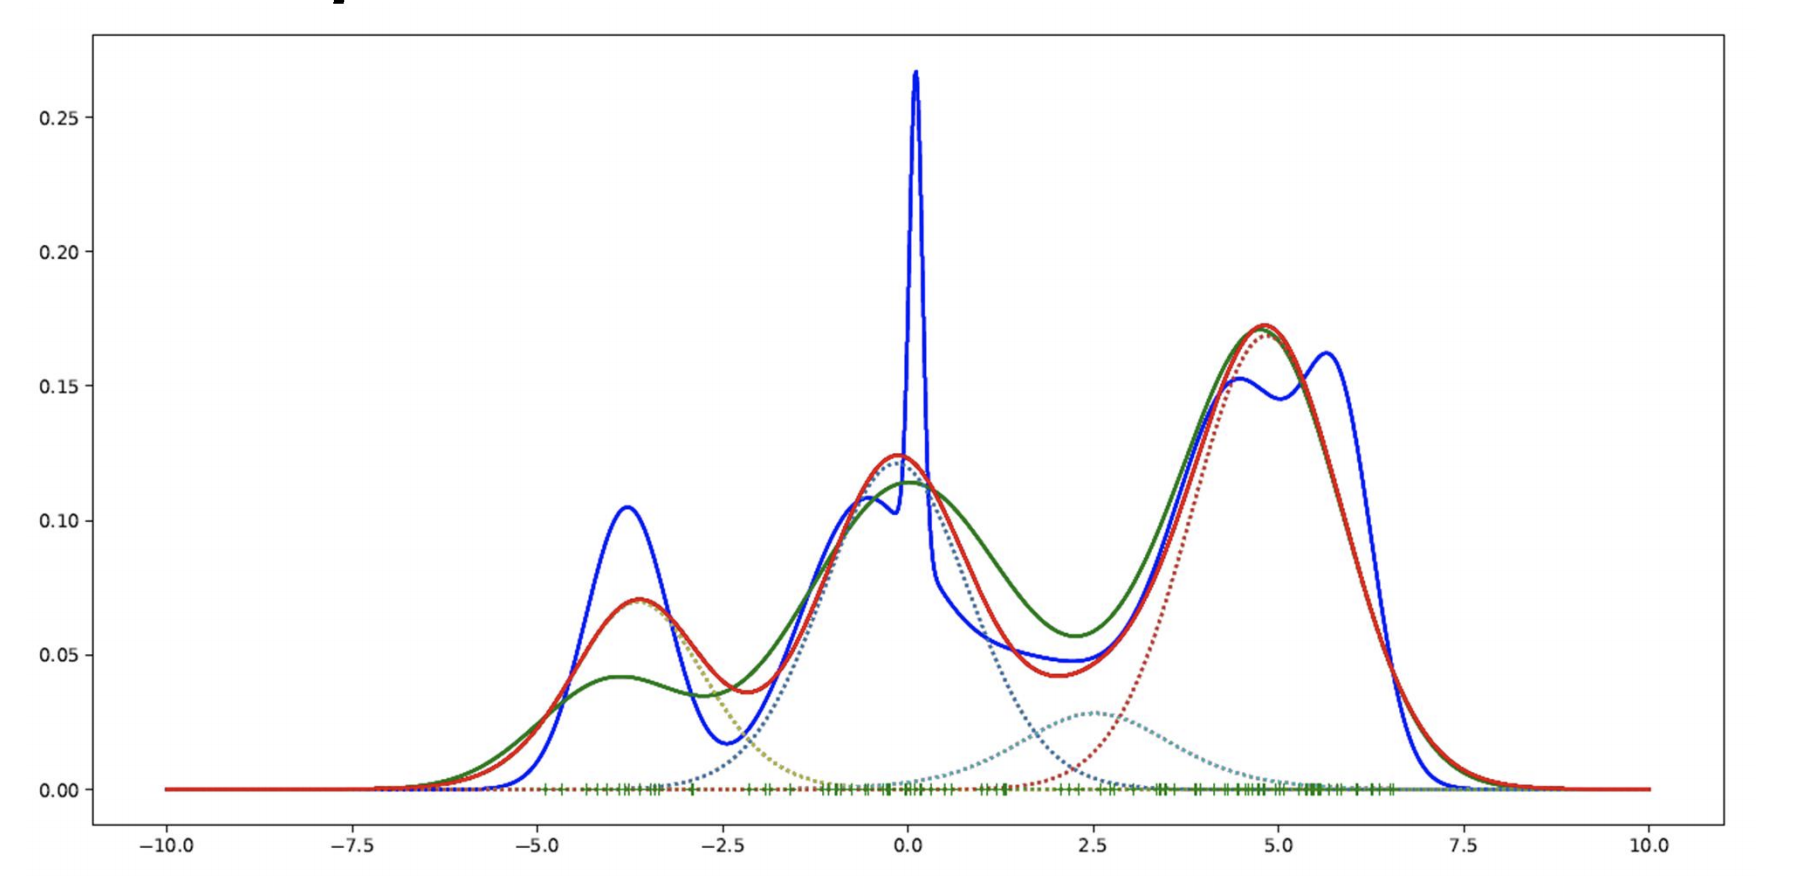
\includegraphics[width=.9\textwidth]{images/ml_vs_vb}
\end{center}
\hfill \tiny{Image Credit: Lukas Burget} \normalsize

\begin{itemize}
\item \red{VB} was initialized from the \blue{ML} solution 
\item \red{VB} recovers from \blue{ML} overfitting and is closer to the \green{true distribution} for generating the training data
\end{itemize}

% Details: http://www.fit.vutbr.cz/~burget/BayesianModels/4-Approximate%20inference.pdf
\end{frame}

\begin{frame}{Extensions of Bayesian Mixture Models}

The Bayesian framework can be used to endow mixture models with many nice properties.
\vfill
\metroset{block=fill}
\begin{block}{Example: Dirichlet Process Mixture Models (DPMMs)}
DPMM's have an unbounded number of mixture components.   \\
\vfill
The model automatically adapts its number of components.

\begin{itemize}
\item Click \blue{\href{https://scikit-learn.org/stable/auto_examples/mixture/plot_concentration_prior.html\#sphx-glr-auto-examples-mixture-plot-concentration-prior-py}{here}} for Demo 1.
\item Click \blue{\href{https://scikit-learn.org/stable/auto_examples/mixture/plot_gmm.html\#sphx-glr-auto-examples-mixture-plot-gmm-py}{here}} for Demo 2.
\end{itemize}
\end{block}



\end{frame}


\subsection{Inference algorithm}
\begin{frame}{Example: Bayesian Gaussian Mixture Model}

To see the mean field CAVI algorithm \eqref{mfcavi_update} in a concrete context, consider a version of the Bayesian Gaussian Mixture Model.  
\begin{align*}
\mu_k & \sim \text{Normal}(M_k = 0, V_k = \sigma^2) && k = 1,..., K\\
c_i & \sim \text{Categorical}(\pi_1, ..., \pi_K) && i=1, ... ,n \\
x_i \cond c_i, \mu & \sim \text{Normal}(\mu_{c_i}, 1) && i = 1,..., n
\end{align*}
\tiny (The model is simple in that it assumes univariate observations and that each mixture component has unit variance.) \normalsize 

The joint density, by chain rule, is
\[ p(x,c,\mu) = p(\mu) \ds\prod_{i=1}^n p(c_i) p(x_i \cond c_i, \mu) \]

And a mean-field variational family is given by 
\[  q(c, \mu) = \ds\prod_{k=1}^K q(\mu_k) \ds\prod_{i=1}^n q(c_i) \]

\end{frame}

\begin{frame}{Example: Bayesian Gaussian Mixture Model}
We apply \eqref{mfcavi_update} to determine the coordinate updates for $q_{c_i}$, the variational factors governing cluster assignments.   %We take the log of the joint density and utilize proportionality to obtain

\begin{align*}
q(c_{ik}) & \propto \exp \bigg\{ \E_{q_{\mu_k}} \bigg[  \log p(c_i =k) + \log p(x_i \cond c_i=k, \mu) \bigg] \bigg\} \\
& \propto \exp \bigg\{ \E_{q_{\mu_k}} \bigg[ \log \pi_k + x_i \mu_k - \df{1}{2} \mu_k^2 \bigg] \bigg\} \\
& \propto \pi_k \exp \bigg\{ x_i \E_{q_{\mu_k}} [\mu_k] - \df{1}{2}  \E_{q_{\mu_k}} [ \mu_k^2] \bigg\} \\
\end{align*}

The next slide reveals that the $q_{\mu_k}$ are Gaussian, and hence the above expectations are easy to compute. 

\vfill
\tiny
\alert{Note:} We abuse notation, and write $q(c_{ik})$ as shorthand for $q(c_i =k)$
\end{frame}

\begin{frame}{Bayesian Gaussian Mixture Model: \\ Updates to mixture component means}
Using the same strategy as when updating cluster assignments $c_i$, we obtain

\begin{align*}
q(\mu_k) & \propto \exp \bigg\{ \E_{-q_{\mu_k}} \bigg[  \log p(\mu_k) + \ds\sum_{i=1}^n \log p(x_i \cond c_i=k, \mu) \bigg] \bigg\} \\
& \propto \exp \bigg\{ -\df{1}{2  \sigma^2} \mu_k^2 +  \ds\sum_{i=1}^{n} \E_{q_c} \bigg[ \+1_{c_i=k}\, \bigg(x_i \mu_k - \df{1}{2} \mu_k^2\bigg) \bigg] \bigg\} \\
& \propto \exp \bigg\{  \bigg( \ds\sum_{i=1}^n q(c_{ik})x_i  \bigg) \mu_k   \; +  \; -\df{1}{2} \bigg(\df{1}{ \sigma^2} + \ds\sum_{i=1}^n q(c_{ik}) \bigg) \mu_k^2 \bigg\} \\
\end{align*}


 
which is an exponential family distribution with sufficient statistics $(\mu_k, \mu_k^2)$  and base measure $\propto 1$; hence it is Gaussian. 

\end{frame}

\begin{frame}{Bayesian Gaussian Mixture Model: \\ Updates to mixture component means}

It is easy to show\footnote{\tiny Indeed, in this course we have seen} that for a Gaussian with mean $M$ and variance $V$, the natural parameters are given by
 \[\eta_1 = \df{M}{V}, \quad \eta_2 = -\df{1}{2V} \]
 
From the last slide, the variational density $q(\mu_k)$ has natural parameters
\[ \eta_1 = \bigg( \ds\sum_{i=1}^n q(c_{ik})x_i  \bigg) , \quad \eta_2 = -\df{1}{2} \bigg(\df{1}{ \sigma^2} + \ds\sum_{i=1}^n q(c_{ik}) \bigg) \]


 
   Using this, we can backsolve to determine the updates to the mean and variance of the Gaussian variational density governing the kth cluster mean:
\[ M_k = \df{\sum_{i=1}^n q(c_{ik}) x_i}{1/\sigma^2 + \sum_{i=1}^n q(c_{ik})}, \quad V_k= \df{1}{1/\sigma^2 +\sum_{i=1}^n q(c_{ik})}\]
\end{frame}

\justfor{long}{
	\section{Tool: CAVI with Exponential Family Complete Conditionals}
	
	\begin{frame}{Motivation}
	
	The form of \eqref{mfcavi_update} suggests that MF-CAVI can be simplified when the complete conditional has known form.  We consider the case where complete conditionals are in the exponential family
	
	This situation describes a lot of models:
	
	\metroset{block=fill}
	\begin{block}{Models with exponential family complete conditionals}
	\begin{itemize}
	\item Bayesian mixture models (where the mixture components are exponential families and conjugate priors are used)
	\item Bayesian Hidden Markov Models (HMMs)
	\item Hierarchical HMMs 
	\item Switching Kalman Filters
	\item Certain hierarchical regression models (Linear regression, Poisson regression, probit regression)
	\item Matrix factorization models
	\item $[...]$
	\end{itemize}
	\end{block}
	
	\end{frame}
	
	\begin{frame}{The Exponential Family} 
	
	We define an \textit{exponential family} of probability distributions as those distributions whose density has the following form
	\begin{align}
	\label{eqn:exponential_family}
	 p(x \cond \eta) = h(x) \exp \{ \eta^T s(x) - a(\eta)\} 
	 \end{align}
	where we refer to $h$ as the base measure, $\eta$ as the natural parameter, $s$ as the sufficient statistics, and $a$ as the log normalizer. 
	\vfill \vfill
	\tiny
	\alert{Note:} $x\perp \!\!\! \perp  \theta \cond t(x)$
	\end{frame}
	
	
	\begin{frame}{MF-CAVI updates on random variables with exponential family complete conditionals}  \label{slide_claim}
	
	\scriptsize
	
	
	\metroset{block=fill}
	\begin{block}{Claim}
	\scriptsize
	Consider a model with unobserved random variables $(u_1,...,u_k)$.  Let 
	
	\begin{enumerate}
	\item Variational density $q$ have mean field factorization $q=q_k(u_k)q_{-k}(u_{-k})$. 
	\item $p(u_k \cond u_{-k}, x)$ be in exponential family $\mathcal{E}$ with natural parameter $\eta_k(u_{-k}, x)$.  
	\end{enumerate}
	
	Then optimal mean field CAVI update \eqref{mfcavi_update} puts
	
	\begin{align}
	\label{eqn:mf_cavi_efcc_0}
	q_k \in \mathcal{E}  
	\end{align}
	
	 with natural parameter 
	
	\begin{align}
	\label{eqn:mf_cavi_efcc}
	\boxed{\nu_k = \E_{q_{-k}} [\eta_k(u_{-k}, x)]}
	\end{align}
	\end{block}
	
	\begin{block}{Take Home}
	\scriptsize 
	\begin{itemize} 
	\item Variational factor is in same family as complete conditional.
	\item Its natural parameter is the expectation \tiny  (with respect to the other variational factors) \scriptsize of the natural parameter of the complete conditional.
	\end{itemize} 
	\end{block}
	%SAY: That is, the optimal update sets the natural variational parameter equal to the expectation (with respect to the other variational factors) of the natural parameter of the complete conditional.
	
	\end{frame}
	
	\begin{frame}{Proof}
	If the $k$th complete conditional is in the exponential family, then we have 
	\begin{align}
	\label{eqn:efcc}
	 p(u_k \cond u_{-k}, x) = h(u_k) \exp \{ \eta_k^T s(u_k) - a(\eta_k)\} 
	 \end{align}
	\tiny Note that our notation suppresses that the natural parameter $\eta_k$ depends on the conditioning variables $(u_{-k}, x)$. \normalsize
	
	By substituting \eqref{eqn:efcc} into \eqref{mfcavi_update} and discarding factors that do not depend on $u_k$, we obtain
	
	\begin{align*}
	q_k(u_k) & \propto  \exp \bigg\{ \E_{q_{-k}} \bigg[  \eta_k^T s(u_k) + \log h(u_k) \bigg] \bigg\} \\
	& \propto  h(u_k) \exp \bigg\{ \E_{q_{-k}}[ \eta_k]^T s(u_k) \bigg\} 
	\end{align*}
	
	Since $h$ and $s$ are identical to those of \eqref{eqn:efcc}, the claim holds. 
	
	\end{frame}
}


\justfor{long}{
\section{Example: Bayesian Hidden Markov Model}

\begin{frame}{Hidden Markov Model}
A  hidden Markov model (HMM) is a tool for representing probability distributions over sequences of observations.  

The HMM assumes that 
\begin{itemize}
\item The observation at time $t$, $y_t$, was generated by some process whose state $x_t$ is hidden from the observer. 
\item The sequence of states satisfies the \textit{Markov property}:  conditional on the current state $x_t$, past and future hidden states are independent. 
\item There is an additional Markov property on outputs:  conditional on the current state $x_t$, the output $y_t$ is independent of all other hidden states and outputs.
\end{itemize}

\end{frame}

\begin{frame}{Notation}
\begin{itemize}
\item $y_{1:T}=(y_1, ..., y_T)$ observed sequence
\item $x_{1:T} =(x_1, ...., x_T)$: hidden state sequence ($x_t \in \{1,...,K \}$) 
\item $\pi = \{ \pi_k \}, \pi_k = P(x_1 = k)$: initial state distribution
\item $A=\{A_{kk'}\}, A_{kk'} = P(x_t= k' \cond x_{t-1}=k):$ state transition probability matrix 
\item $\phi = (\phi_k)_{k=1}^K$ a set of parameters, each governing an output distribution (also called emissions distribution) associated to each hidden state; that is, $ P(y_t \cond x_t=k) = P(y_t \cond \phi_k)$. 
\item $\theta = (\pi, A, \phi)$: model parameters
\end{itemize}
\end{frame}


\begin{frame}{HMM: Complete Data Likelihood (CDL) }
The complete data likelihood for the HMM is given by 
\begin{align}
 p(x_{1:T}, y_{1:T} \cond \theta) &=  p(x_1 \cond \theta)  p(y_1 \cond x_1, \theta) \ds\prod_{t=2}^T p(x_t \cond x_{t-1}, \theta) p(y_t \cond x_t, \theta) \nonumber \\
 &=  p(x_1 \cond \pi) p(y_1 \cond x_1, \phi) \ds\prod_{t=2}^T p(x_t \cond x_{t-1}, A) p(y_t \cond x_t, \phi)   \nonumber \\
 &= \pi_{x_1}  \; \ds\prod_{t=2}^T A_{x_{t-1}, x_t} \ds\prod_{t=1}^T p(y_1 \cond \phi_{x_t}) \label{eqn:hmm_cdl_compact}
 \end{align}
\end{frame}

\begin{frame}{HMM: Complete Data Likelihood is an Exponential Family}
We continue 
\small
\begin{align}
p(x_{1:T}, y_{1:T} \cond \theta) &=  \exp\bigg \{ \log p(x_1 \cond \pi) + \ds\sum_{t=2}^T \log p(x_t \cond x_{t-1}, A) +  \ds\sum_{t=1}^T \log p(y_t \cond x_t, \phi) \bigg\}  \nonumber \\
&= \exp \bigg \{ \log \pi_{x_1}  + \ds\sum_{t=2}^T \log A_{x_{t-1}, x_t} + \ds\sum_{t=1}^T \log p(y_1 \cond \phi_{x_t}) \bigg\} \label{eqn:hmm_cdl_ef_compact} \\
&=  \exp\bigg \{  \ds\sum_{k=1}^K x_1^k \log \pi_k + \ds\sum_{t=2}^T \ds\sum_{k, k'=1}^K x_{t-1}^k x_t^{k'} \log A_{kk'} \nonumber \\ 
&\quad\quad\quad\quad\quad  + \ds\sum_{t=1}^T \ds\sum_{k=1}^K x_t^k \log p(y_t \cond x_t, \phi_k)  \bigg\} \label{eqn:hmm_ef_form}
\end{align}

\tiny where we have defined
\[ x_t^k =  
\begin{cases}	  
1, & \text{if the latent state at time $t$ is $k$} \\
0, & \text{otherwise}
\end{cases} \]

\small

Thus, the complete data likelihood \tiny (although not the marginal  likelihood $p(x_{1:T} \cond \theta)$) \normalsize is in the exponential family, so long as the emissions distributions are.   The sufficient statistics for $\log \pi_k$ are $x_1^k$, and the sufficient statistics for $\log A_{kk'}$ are $\sum_{t=2}^T x_{t-1}^k x_t^{k'}$.

%\vfill \vfill
%\tiny
%\hfill \alert{Note:} The \textit{marginal} likelihood $p(x_{1:T} \cond \theta)$ is \textit{not} in the exponential family.  
\end{frame}


\begin{frame}{Prior Distributions}
Let us impose a prior whose density factorizes as follows
\begin{align}
\label{eqn:bayesian_hmm_prior_macro}
p(\theta) &= p(A) p(\phi) p(\pi) 
 \end{align}
and let us further assume that the priors have the form
\begin{align}
p(\pi) &= \text{Dirichlet}(\pi \cond \alpha^\pi) \label{eqn:bayesian_hmm_prior_pi}  \\
p(A) &= \ds\prod_{k=1}^K p(A_k \cond \alpha^{A_k}) =  \ds\prod_{k=1}^K \text{Dirichlet}(A_k \cond \alpha^{A_k}) \label{eqn:bayesian_hmm_prior_transition} 
\end{align}
where $A_k$ designates the $k$th row of $A$. 
\end{frame}

\begin{frame}{$\pi$ has a Dirichlet complete conditional}
By the structure of the complete data likelihood \eqref{eqn:hmm_ef_form} and prior \eqref{eqn:bayesian_hmm_prior_macro}, \eqref{eqn:bayesian_hmm_prior_pi} ,  we see that the complete conditional of $\pi$ is a Dirichlet
\begin{align*}
p(\pi \cond \theta_{-\pi}, x_{1:T}, y_{1:T} ) & \propto p(\pi, \theta_{-\pi},  x_{1:T}, y_{1:T}) \\
&\propto \exp \bigg\{ \ds\sum_{k=1}^K  (\alpha_{k}^\pi -1) \log \pi_k \bigg\}  \exp \bigg\{  \ds\sum_{k=1}^K   x_{1}^k \log \pi_k  \bigg\}  \\
&\propto \exp \bigg\{ \ds\sum_{k=1}^K  \bigg( \alpha_k^\pi -1 + x_1^k \bigg) \log \pi_k   \bigg\}  
\end{align*}
since this is an exponential family with base measure $h(\pi) \propto 1$ and the sufficient statistics are $\log \pi  = [\log \pi_1, ..., \log \pi_K]^T$.      
\end{frame}

\begin{frame}{Variational update for $\pi$}
From the last slide, the natural parameter for the complete conditional for $\pi$ is given by 
\[ \eta^{\pi} =
 \begin{bmatrix} 
\alpha_1^\pi -1 + x_1^1\\
... \\
\alpha_K^\pi  -1 + x_1^k \\
 \end{bmatrix}
 \]

Let us assume the factorization $q(A,\phi,\pi, z) = q(\phi, A, z)q(\pi)$.  

Then 
we can apply our Claim (Slide \ref{slide_claim}) to discover that the optimal MF-CAVI update takes $q(\pi)$ to be Dirichlet with variational natural parameter 

\[  \nu^{\pi} = \E_{q_{-\pi}} [\eta^{\pi}]=
 \begin{bmatrix} 
\alpha_1^\pi  -1 +  \E_{q_x} [x_1^1 ] \\
... \\
\alpha_K^\pi  -1 +   \E_{q_x} [x_1^K] \\
 \end{bmatrix}
 = \alpha^\pi + \E_{q_x} [x_1]  \]
\end{frame}

\begin{frame}{The rows of $A$ have Dirichlet complete conditionals}The updates for the rows $A_k$ can be determined using a similar argument as for $\pi$.   By the structure of the complete data likelihood \eqref{eqn:hmm_ef_form} and prior \eqref{eqn:bayesian_hmm_prior_macro}, \eqref{eqn:bayesian_hmm_prior_transition}, we see that the complete conditional of $A_k$ is also Dirichlet 
% For below, the complete conditional is proportional to the joint, and we only need to worry about the terms $A_k$.
\begin{align*}
p(A_k & \cond \theta_{-A_k}, x_{1:T}, y_{1:T} ) \propto p(A_k, \theta_{-A_k},  x_{1:T}, y_{1:T}) \\
&\propto \exp \bigg\{ \ds\sum_{k'=1}^K  (\alpha_{k'}^{A_k} -1) \log A_{kk'} \bigg\}  \exp \bigg\{  \ds\sum_{k'=1}^K \ds\sum_{t=2}^T  x_{t-1}^k x_t^{k'} \log A_{kk'}  \bigg\}  \\
&\propto \exp \bigg\{ \ds\sum_{k'=1}^K  \bigg( (\alpha_{k'}^{A_k} -1) + \ds\sum_{t=2}^T  x_{t-1}^k x_t^{k'}  \bigg) \log A_{kk'}   \bigg\}  
\end{align*}
since this is an exponential family with base measure  $h(A_k) \propto 1$ and sufficient statistics  $\log A_k  = [\log A_{k1}, ..., \log A_{kK}]^T$. 

\end{frame}


\begin{frame}{Variational update for $A_k$}
From the last slide, the natural parameter for the complete conditional for $A_k$ is given by 
\small
\[ \eta^{A_k} =
 \begin{bmatrix} 
(\alpha_1^{A_k} -1) + \ds\sum_{t=2}^T x_{t-1}^k x_t^{1} \\
... \\
(\alpha_K^{A_k} -1) + \ds\sum_{t=2}^T x_{t-1}^k x_t^{K} \\
 \end{bmatrix}
 \]
\normalsize
Let us assume factorization $q(A,\phi,\pi, z) = q(\phi, \pi, z) \prod_{k=1}^K q(A_k)$.
 
Then we can apply our Claim (Slide \ref{slide_claim}) to discover that the optimal MF-CAVI update takes $q(A_k)$ to be Dirichlet with variational natural parameter 
\small 
\[  \nu^{A_k} = \E_{q_{-A}} [\eta^{A_k}]=
 \begin{bmatrix} 
(\alpha_1^{A_k}  -1) + \ds\sum_{t=2}^T \E_{q_x} [ x_{t-1}^k x_t^{1} ] \\
... \\
(\alpha_K^{A_k}  -1) + \ds\sum_{t=2}^T  \E_{q_x} [ x_{t-1}^k x_t^{K}] \\
 \end{bmatrix}  
 =  \alpha^{A_k}  + \ds\sum_{t=2}^T \E_{q_x} [x_{t-1}^k x_t] 
  \]

\end{frame}

\begin{frame}{Variational update for $x$}
By applying \eqref{mfcavi_update} and substituting in the form of the complete data likelihood \eqref{eqn:hmm_cdl_compact}, we obtain 

\small
\begin{align*}
q(x) & \propto \exp \bigg\{ \E_{-q(z)} \big[ \log p(x_{1:T}, y_{1:T}, \theta) \big] \bigg\} \\
 &\propto \exp \bigg\{ \E_{q(\pi)} \log \pi_{x_1} \bigg\} \ds\prod_{t=2}^T \exp \bigg\{  \E_{q(A)}   \log A_{x_{t-1}, x_t} \bigg\} \ds\prod_{t=1}^T \exp \bigg\{  \E_{q(\phi)} p(y_1 \cond \phi_{x_t})  \bigg\}
\end{align*}
\normalsize 

Compare this to the original complete data likelihood \eqref{eqn:hmm_cdl_compact}. The structure is identical if we define the alterations  $(A, \pi, p) \to (A^*, \pi^*, p^*)$.

\end{frame}

\begin{frame}
In particular, we define 
\begin{align*}
\pi^* &= \{ \pi^*_k \}_{k=1}^K : \pi^*_k =\exp \bigg\{ \E_{q(\pi)} \log \pi_{x_1} \bigg\} = \exp \bigg\{  \psi(\nu_k^\pi) - \psi(\ds\sum_{j=1}^K \nu_j^\pi) \bigg\} \\
A^* &= \{A_{kk'}^* \}_{k,k'=1}^K : A_{kk'}^*  = \exp \bigg\{  \E_{q(A)}   \log A_{kk'} \bigg\} = \exp \bigg\{   \psi(\nu_{k'}^{A_k}) - \psi(\ds\sum_{j=1}^K \nu_j^{A_k}) \bigg\} \\
p^* &= \{ p^*( \cdot \cond \phi_k) \}_{k=1}^K : p^*_k \propto \exp \bigg\{ \E_{q(\phi_k)} \log p( \cdot \cond \phi_k)\bigg\}
\end{align*}
\tiny $\psi(\cdot)$ is the digamma function; the expectation of the log of a component of a Dirichlet-distributed probability vector is well-known. \normalsize 

Then we can use the forward-backwards algorithm (FBA) to update $q(x)$.
\begin{itemize}
\item A standard HMM applies FBA to $(A, \pi, p)$ in order determine the marginals $p(x_t \cond y, \theta)$ and pairwise marginals $p(x_{t-1},x_t \cond y, \theta)$.
\item Likewise, we can apply FBA to $(A^*, \pi^*, p^*)$ to determine the marginals $q(x_t)$ and pairwise marginals $q(x_{t-1}, x_t)$ \tiny (which, as we have seen, are sufficient for performing the other updates).
\end{itemize}

\end{frame}
}

\section{Example: Latent Dirichlet Allocation (LDA)}

\begin{frame}{Acknowledgements}

This section, especially the intro, borrows heavily from David Blei's 2012 ICML tutorial. 

\end{frame}


%%%%%%%%%%%%%%%%%%%%%%%%%%%%%%%%%%%%%%%%%%%
\begin{frame}{Overview}

LDA is a generative probabilistic model of a corpus of documents of text.  \\
\vfill
LDA assumes:

\begin{itemize}
\item There is a set of \alert{topics} that describe the corpus
\item Each document exhibits these topics to varying degrees.  % (each word in a document was generated by one of these topics.).
\end{itemize}
\vfill
\pause 

So:
\begin{itemize}
\item The topics and how they relate to the documents are hidden structure
\item The main computational problem is to infer this hidden structure 
\end{itemize}
\end{frame}


%%%%%%%%%%
\begin{frame}

\begin{center}
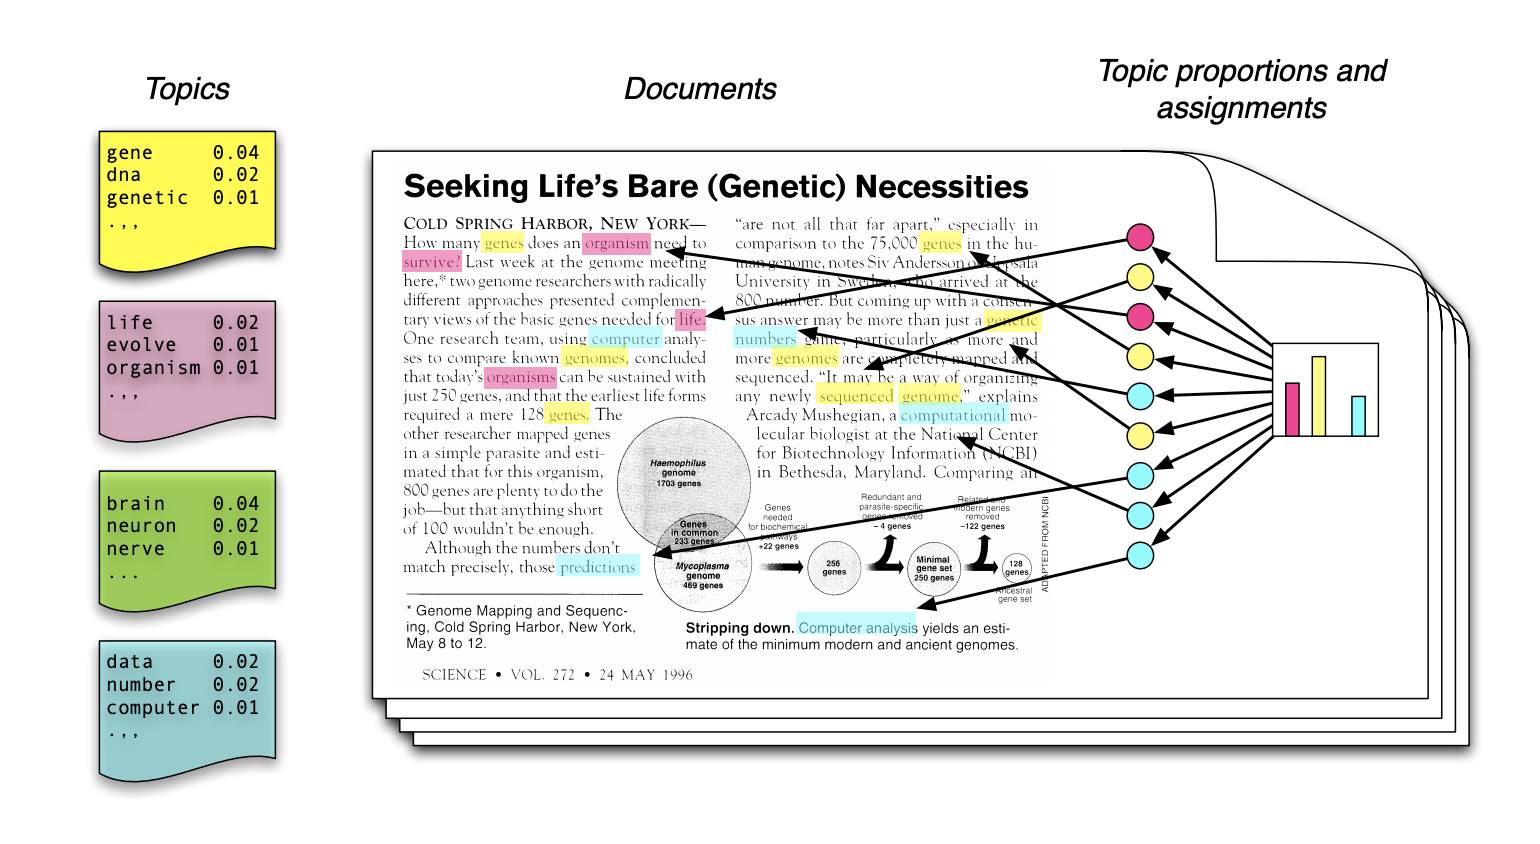
\includegraphics[width=\textwidth]{images/lda_intro}
\end{center}


\begin{itemize}
\item Each \textbf{topic} is a distribution over words. \pause
\item Each \textbf{document} is a mixture of corpus-wide topics. \pause
\item Each \textbf{word} is drawn from one of those topics. \pause
\end{itemize}

\pause 
\vfill  \vfill \vfill


\tiny  \bf{Rk:}  This is a ``bag of words" model. \\
\pause
\hfill \tiny Source: David Blei, 2012 ICML Tutorial \normalsize
\end{frame}


%%%%%%%%%%%%%%
\justfor{long}{
	\begin{frame}{LDA as Probabilistic Matrix Factorization}
	\footnotesize
	The matrix of word frequencies across the corpus decomposes as
	
	\begin{center}
	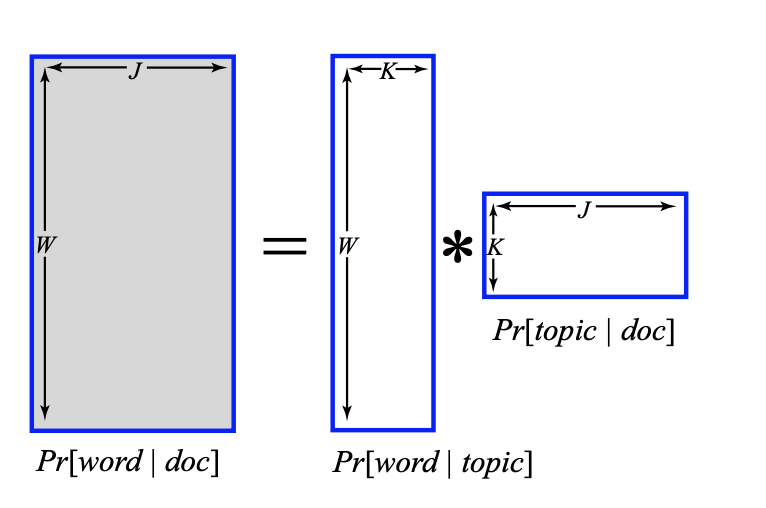
\includegraphics[width=.9\textwidth]{images/lda_as_probabilistic_matrix_factorization}
	\end{center}
	
	\scriptsize
	LDA can be seen as a probabilistically constrained factorization of the matrix describing the bag of words composing each group, or document.  \\
	\vfill
	The number $K$ of latent topics determines the factorization’s rank.  \\
	\vfill
	% The hyperparameters $\alpha$ and $\beta$ define Dirichlet priors for
	%the columns of the topic and word distribution matrices, respectively \
	
	\hfill \tiny Image Credit : Erik Sudderth
	
	\end{frame}
}
%%%%%%%%%%
\begin{frame}

\begin{center}
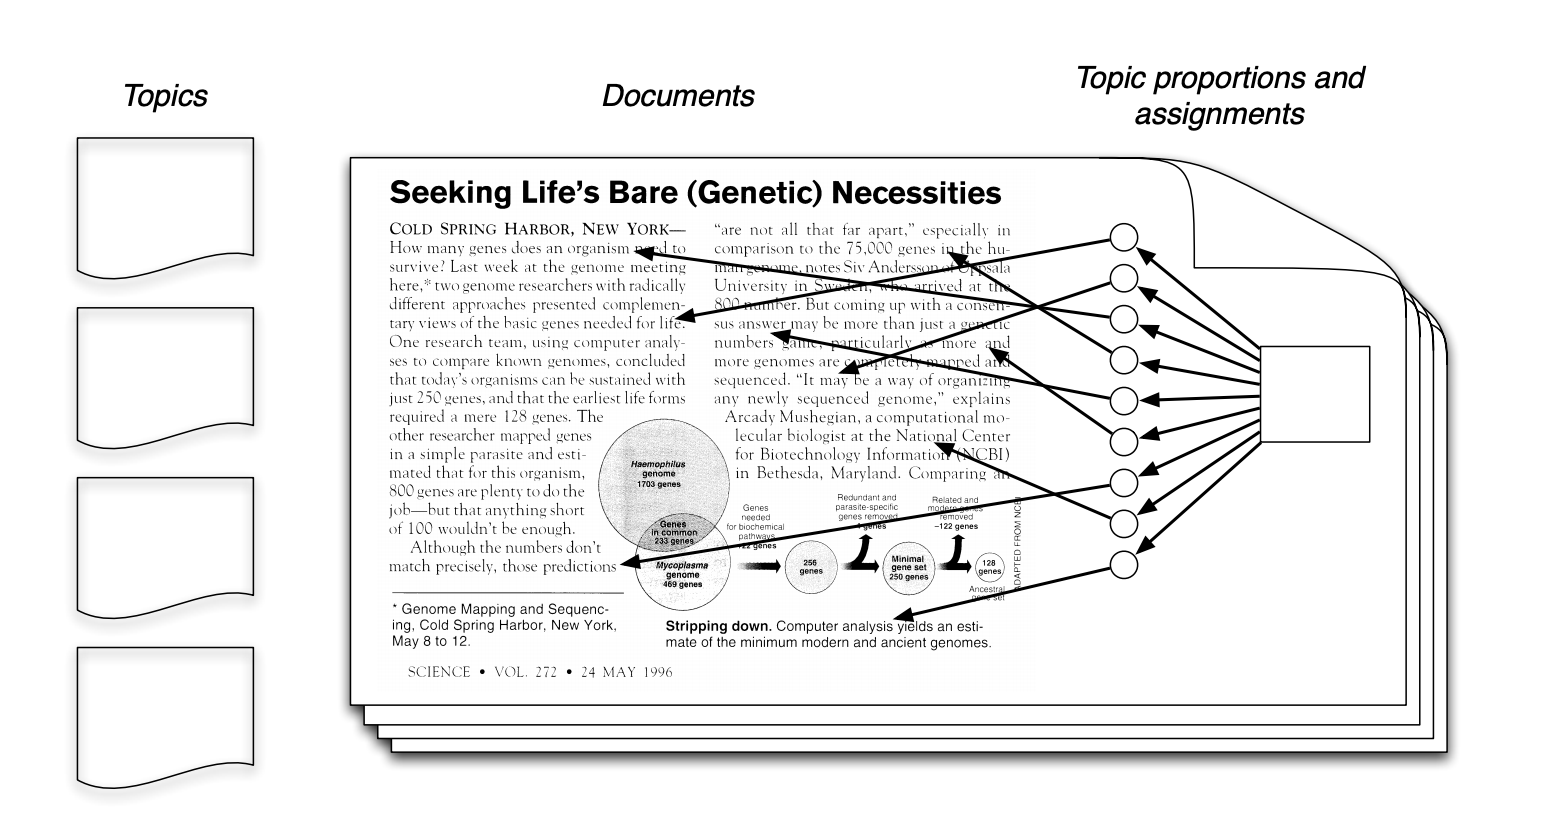
\includegraphics[width=\textwidth]{images/lda_intro_2}
\end{center}


\begin{itemize}
\item In reality, we only observe the documents. \pause 
\item The model structure is \textbf{hidden}. \pause
\item Our goal is to \textbf{infer} the hidden variables; i.e. compute 
\[ p(\text{topics, proportions, assignments} \cond \text{documents} ) \]
\end{itemize}

% \hfill \tiny Source: David Blei, 2012 ICML Tutorial \normalsize
\end{frame}


%%%%%%%%%%
\begin{frame}{Recall: Dirichlet Distribution}

\begin{itemize}
\item Dirichlet distribution is \textit{conjugate prior} of Categorical
\[  p(\theta \cond \alpha)  = \df{\Gamma (\sum_{i=1}^K \alpha_i)}{ \prod_{i=1}^k \Gamma(\alpha_i)}  \theta_1^{\alpha_1 -1 } \cdots  \theta_k^{\alpha_k -1 }  \]
\pause 
\item For symmetric Dirichlet distributions ($\alpha_1 = ... = \alpha_K$),  a scalar hyperparameter $\alpha = \sum_k \alpha_k$ controls the shape and sparsity of the $\theta_d$'s. \tiny(per-document topic proportions) \normalsize .   
	\begin{itemize}
	\item high $\alpha$:  typical $\theta_d$ \tiny (from the prior) \normalsize will be uniform
	\item small $\alpha$: a typical $\theta_d$ \tiny (from the prior) \normalsize will be sparse
	\end{itemize}
	\begin{center}
	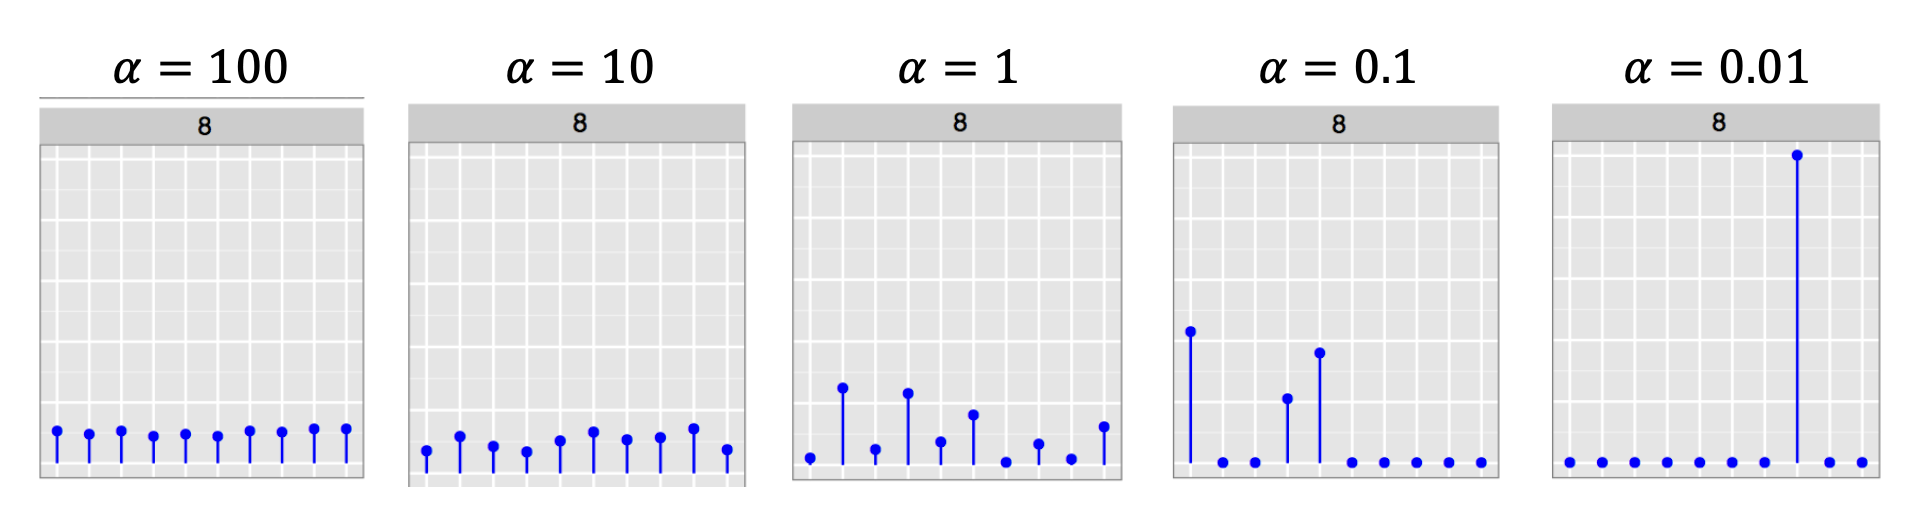
\includegraphics[width=.8\textwidth]{images/dirichlet_role_of_hyperparameter}
	\end{center} 
\pause 
\item Likewise, $\eta$ controls the shape and sparsity of the $\beta_k$'s \tiny(the topics -- distribution over words) \normalsize
\end{itemize}
\end{frame}



%%%%%%%%%%
\begin{frame}{LDA: Generative Process}
\footnotesize
The model is described by the following \bf{generative process}:
\pause 
\begin{itemize}
\item Fix a vocabulary of $V$ words, and set the number of topics,  $K$.  \pause 
\item Set hyperparameters $\eta \in \R^V, \alpha \in \R^K$. \pause 
\item For $k$ in $(1,K)$:
	\begin{itemize}
	\item Define the \textit{topic} \tiny (a distribution over words),  \footnotesize $\beta_k \in \R^V \sim \text{Dir}(\eta)$.\footnote{\tiny Interpretation of $\eta$: psuedocount of vocabulary words observed across prior topics.} \pause 
	\end{itemize}
\item For $d$ in $(1,D):$
	\begin{itemize}
	\item Choose  \tiny (per-document)  \footnotesize \textit{topic proportions}   $\theta_d \in \R^K \sim \text{Dir}(\alpha)$.\footnote{\tiny Interpretation of $\alpha$: psuedocount of topics observed across prior documents.} \pause 
	\item For $n$ in $(1, N_d)$:
		\begin{itemize}
		\item Choose the \textit{topic assignment} $\alert{z_{d,n}} \sim \text{Categorical}_K (\theta_d)$ \pause
		\item Choose \textit{word} $w_{d,n} \sim \text{Categorical}_V(\beta_{\alert{z_{d,n}}})$
		\end{itemize}
	\end{itemize}
\end{itemize}
\end{frame}


%%%%%%%%%%%
%\begin{frame}{LDA: Generative Process}
%\footnotesize
%
%\begin{itemize}
%\item Choose the vocabulary of $V$ words, and set the number of topics,  $K$. 
%\item Set hyperparameters $\eta \in \R^V, \alpha \in \R^K$.
%\item For $k$ in $(1,K)$:
%	\begin{itemize}
%	\item Choose \textit{per-topic word distribution} $\beta_k \in \R^V \sim \text{Dir}(\eta)$.\footnote{\tiny Interpretation of $\eta$: psuedocount of vocabulary words observed across prior topics.}
%	\end{itemize}
%\item For $d$ in $(1,D):$
%	\begin{itemize}
%	\item Choose  \textit{per-document topic distribution}   $\theta_d \in \R^K \sim \text{Dir}(\alpha)$.\footnote{\tiny Interpretation of $\alpha$: psuedocount of topics observed across prior documents.}
%	\item For $j$ in $(1, N_d)$:
%		\begin{itemize}
%		\item Choose \textit{topic} $z_{d,n} \sim \text{Categorical}_K (\theta_d)$
%		\item Choose \textit{word} $w_{d,n} \sim \text{Categorical}_V(\beta_{z_{d,n}})$
%		\end{itemize}
%	\end{itemize}
%\end{itemize}
%\end{frame}





%%%%%%%%%%
\begin{frame}{LDA as a graphical model}

\begin{center}
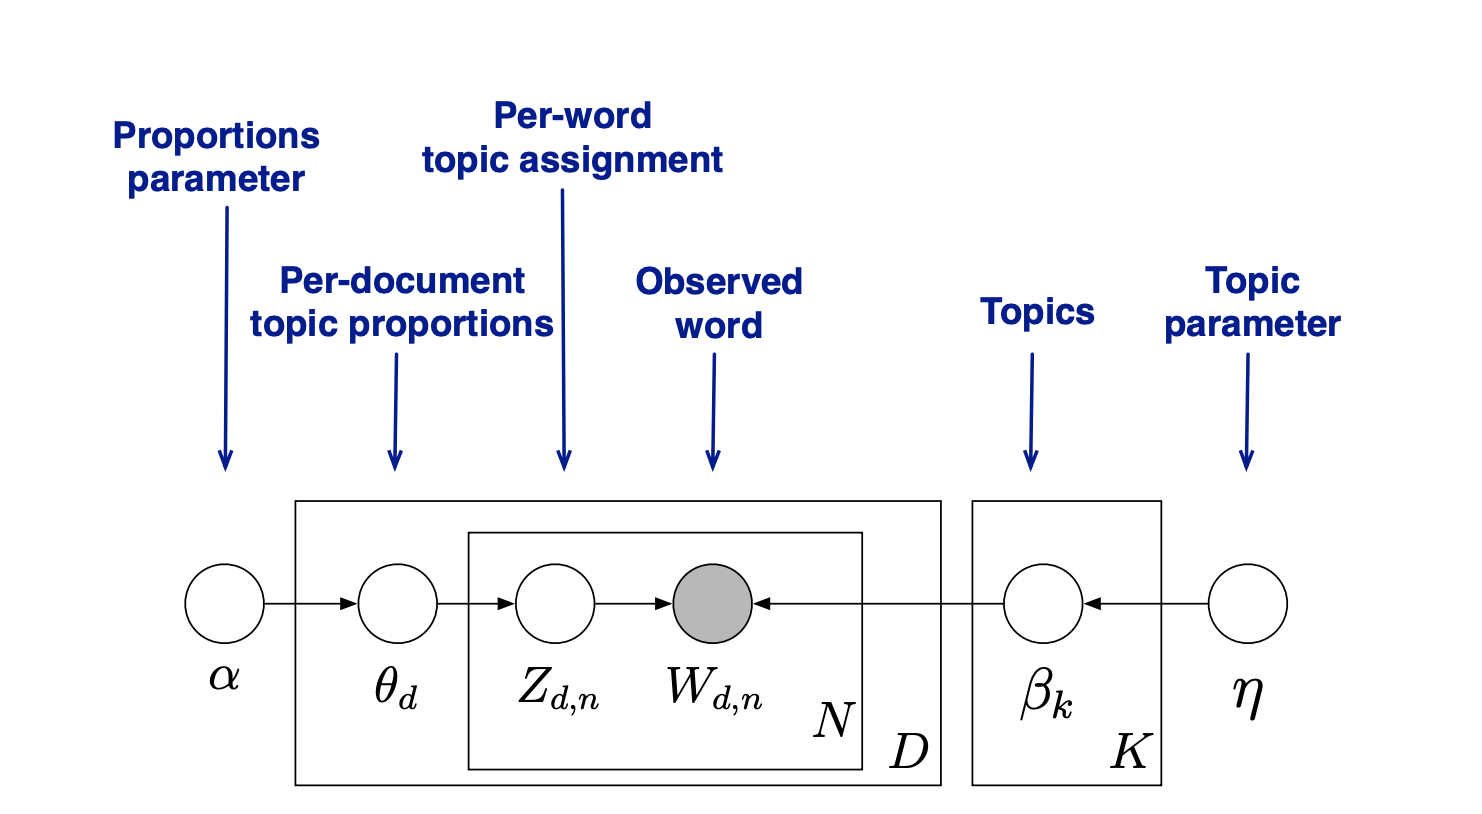
\includegraphics[width=\textwidth]{images/lda_graphical_model}
\end{center}

Recall:
\scriptsize
\begin{itemize}
\item Nodes are random variables. 
\item Shaded nodes are observed.
\item Plates indicate replicated variables.
\item Each node is conditionally independent from its non-descendants given its parents.
\end{itemize}
\end{frame}


%%%%%%%%%%
\begin{frame}{Joint distribution}

\begin{center}
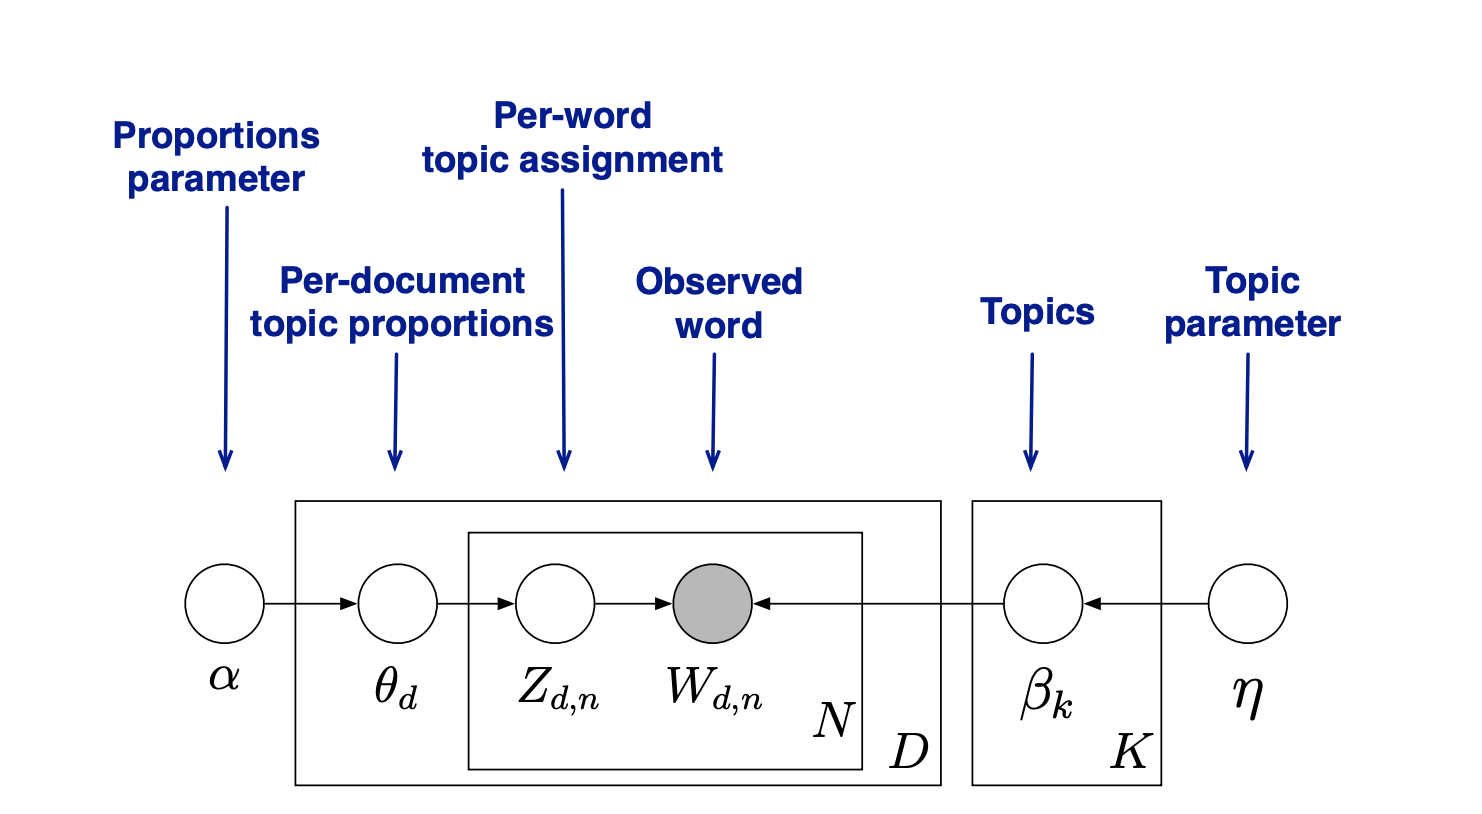
\includegraphics[width=.9\textwidth]{images/lda_graphical_model}
\end{center}

\footnotesize
\begin{equation}
p(\+z, \+\theta, \+w, \+\beta \cond \+\alpha, \+\eta)  = \ds\prod_{k=1}^K \explainterm{Dirichlet}{p(\+\beta_k \cond \+\eta)}  \ds\prod_{d=1}^D \explainterm{Dirichlet}{p(\+\theta_d \cond \+\alpha)} \; \ds\prod_{n=1}^N \explainterm{Categorical}{p(\+z_{d,n} \cond \+\theta_d)} \; \explainterm{Categorical}{p(\+w_{d,n} \cond \+z_{d,n}, \+\beta_k)}
\label{lda_joint}
\end{equation}
\pause
\vfill 
\tiny \textbf{Remark.} Note that LDA is a ``bag-of-words" model; i.e. the probability of a word (or document) is invariant to word order.
\end{frame}



\begin{frame}{Variational distribution}

We approximate the posterior $p(\+\theta \cond \+z, \+w)$
using mean field variational inference  \eqref{mean_field}. In particular, we assume that the variational family $\Q$ has a density which factorizes as

\begin{align} 
q &= q_\+\delta (\+\theta) \; q_\+\tau (\+z) \nonumber \\
&=  \ds\prod_{d=1}^D \explaintermbrace{Dirichlet}{q_\+\delta (\+\theta_d)}  \; \ds\prod_{n=1}^{N_d} \; \explaintermbrace{Categorical}{q_{\+\tau_n} (\+z_{d,n})} \label{mean_field_lda}
\end{align}

\vfil \vfill \vfill
\tiny \bf{Note} We are treating the topics $\beta_k$ as a constant for simplicity.   For a fuller treatment, see Blei, D. M., Ng, A. Y., \& Jordan, M. I. (2003). Latent dirichlet allocation. Journal of machine Learning research, 3(Jan), 993-1022.
\end{frame}



\begin{frame}{Update equations} 

\metroset{block=fill}
\begin{block}{LDA coordinate ascent update equations}
\begin{align} 
\explainterm{var. dirichlet (topic proportion)}{\delta_{d,k}} &= \explainterm{prior counts}{\alpha_k} + \ds\sum_{n=1}^{N_d} \;\; \explainterm{var. expected assignment}{\tau_{d, n,k}} \label{dirichlet_update} \\
\explainterm{var. categorical (topic assigment)}{\tau_{d,n,k}} &\propto   \explainterm{var. "prior" \; topic assignment}{\exp \bigg\{ \biggE{q_\delta(\theta)}{\log \+\theta_{d,k}} \bigg\} } \;\; \explainterm{likelihood}{\beta_{k, [w_{d,n}]}}  \nonumber  \\
 &= \bigg( \Psi(\delta_k) - \Psi (\ds\sum_j \delta_j) \bigg) \;\;  \beta_{k, [w_{d,n}]} 
 \label{multinomial_update} 
\end{align}

where $\Psi(\cdot)$ is the first derivative of the $\log \Gamma$ function. 
\end{block}


\begin{itemize}
\item Derivable via VBEM (see notes). 
\item Characteristic form: latent variable update depends on the data, global parameter update depends on the latent variable
\end{itemize}

\vfil \vfill \vfill
\tiny \bf{Note} We are treating $\beta$ as a constant for brevity.  We could fit also $\beta$ to the data via  VEM.  (VEM does "empirical Bayes" for you.)   More generally, we could model $\beta$ as a random variable with VBEM.  For a fuller treatment, see Blei, D. M., Ng, A. Y., \& Jordan, M. I. (2003). Latent dirichlet allocation. Journal of machine Learning research, 3(Jan), 993-1022.
\end{frame}


%%%%%%%%%%%%%%%%%%%
\begin{frame}{The role of analytical computations}

The varational categorical update crucially hinges on facts about the \alert{exponential family}.   \pause

In particular, the meat of the proof of the variational categorical update depends crucially on the fact that the Dirichlet of a single probability component is given by
\begin{equation} \label{dirichlet_expect_prob_component}
 \biggE{q_\delta(\theta)}{\log \+\theta_i} =    \Psi(\delta_{i}) - \Psi (\ds\sum_k \delta_k) 
\end{equation}
where $\Psi(\cdot)$ is the first derivative of the $\log \Gamma$ function.  \tiny This fact is justified via facts about the exponential family (such as that the derivative of the log normalization factor with respect to the natural parameter is equal to the sufficient statistic). \normalsize
\vfill
\pause 
For many more complicated models (e.g. VAE), such expectations  \tiny (even the variational ones) \normalsize are intractable, and so we won't be able to use CAVI.
\end{frame}

\begin{frame}{LDA Example Inference}

\scriptsize
\begin{itemize}
\item \textbf{Data}: 17K Science documents from 1990-2000 ( 11M words, 20K unique terms)
\item \textbf{Model}: 100-topic LDA model, fit using variational inference
\end{itemize}

\begin{center}
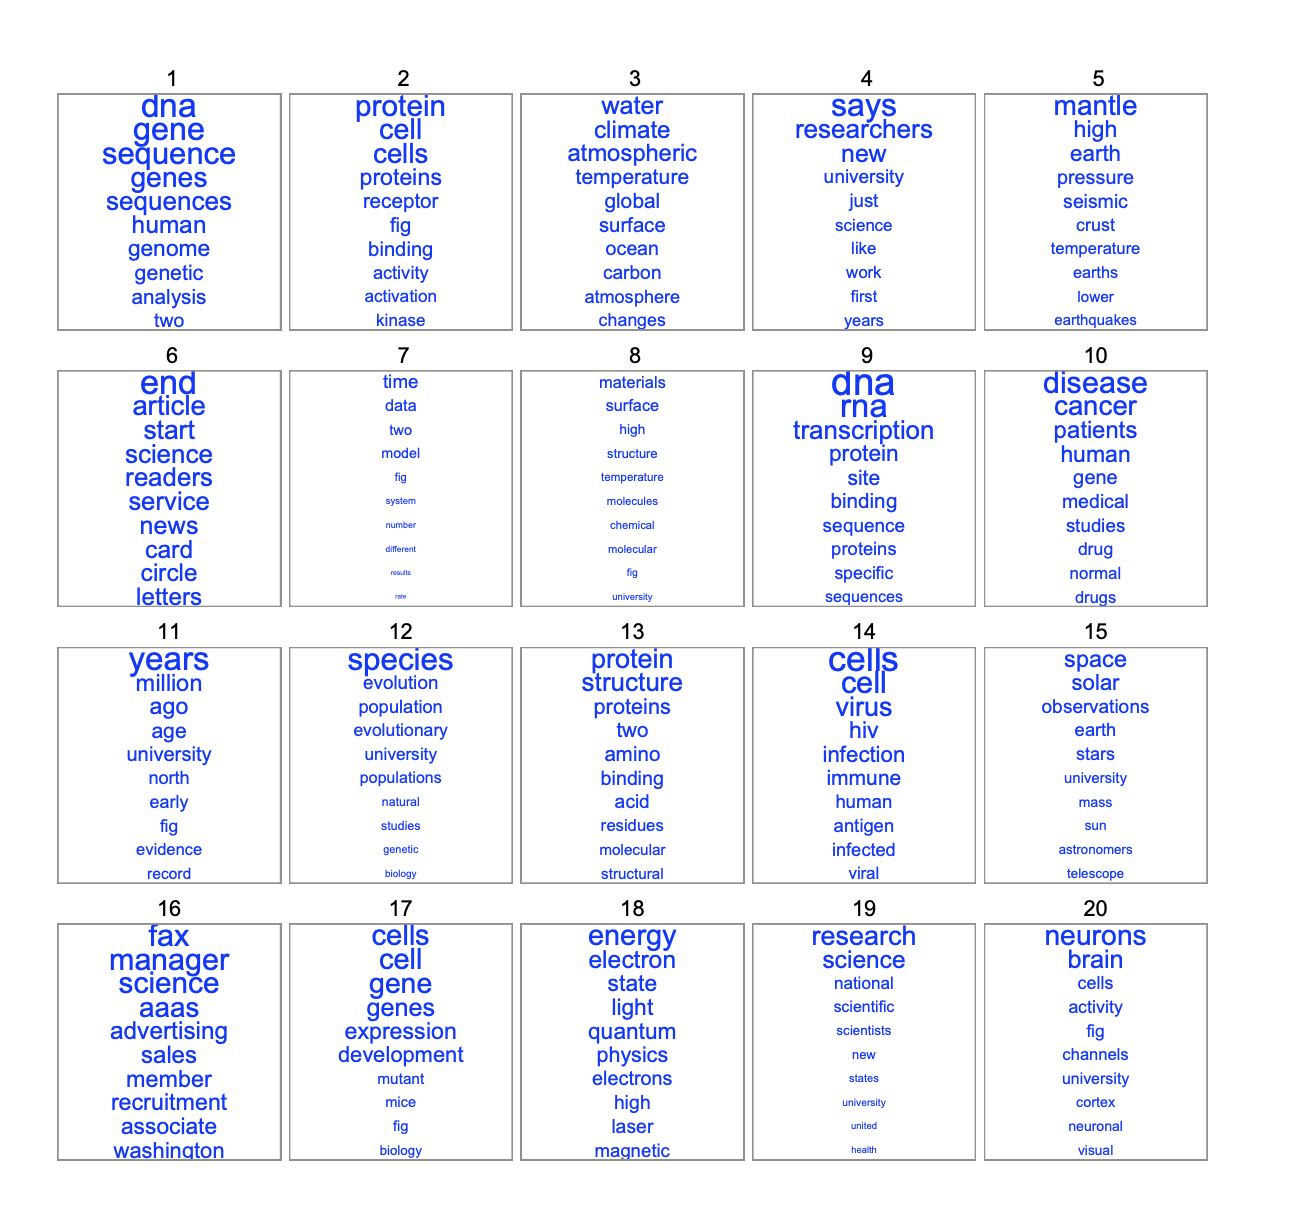
\includegraphics[width=.75\textwidth]{images/lda_example_inference}
\end{center}


\end{frame}


\begin{frame}{Application: Anomaly Detection in Network Traffic Traces }

LDA can be applied to  \textit{documents} that can be just about anything!

\metroset{block=fill}
\begin{block}{IP Addresses}
An \bf{ip address}, like 72.194.113.177, is (roughly) an address assigned to each device connected to the Internet.   My laptop has one, my iphone has one, every website (Google, Apple, etc.) has one, etc. 
\end{block}

One application \tiny (Newton, B. D. (2012). Anomaly Detection in Network Traffic Traces Using Latent Dirichlet Allocation.) \normalsize 
\begin{itemize}
\item ``Documents"  =  the  session of a specific IP address
\item “words” = the full external IP address and port number
combinations. 
\item The “words” in each “document” are counted
and then this data set is processed by LDA to yield a compact
model of the data.
\end{itemize}

\vfill
\tiny \bf{Q:} Ok, but how to perform anomaly detection?
\tiny \bf{Q:} What assumptions are being made by LDA?
\end{frame}

\begin{frame}

\begin{quote}
I analyzed each of the anomalies detected in the last half
hour of the trace [...].  The second anomaly with nearly 300
thousand messages exchanged with an SMTP server, is a bit
more troubling. It is possible that this was actually a malicious
client participating in a Mailbomb attack. According to the
DARPA Intrusion Detection Attacks Database [8] a Mailbomb
attack ``is one in which the attacker sends many messages to
a server, overflowing that server’s mail queue and possibly
causing a system failure.” 
\end{quote}

\end{frame}


%\begin{frame}{Example Inference}
%%
%\begin{minipage}
%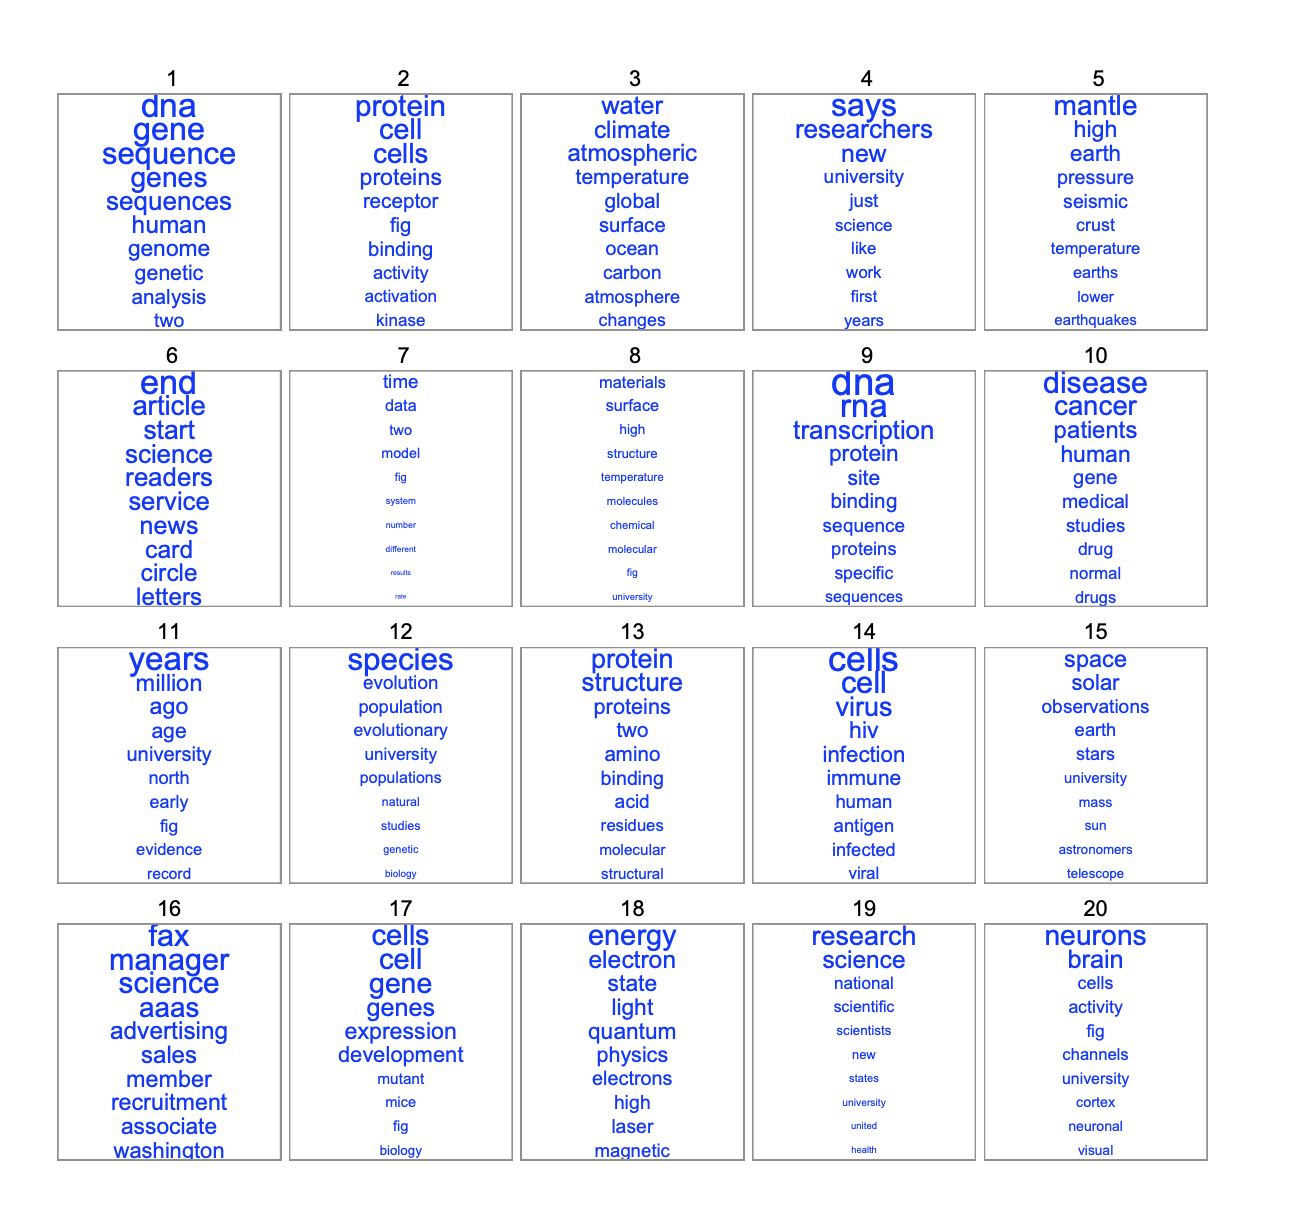
\includegraphics{images/lda_example_inference}
%\end{minipage}
%%%\hfill
%%\begin{minipage}{width=.2\textwidth}
%%\scriptsize
%%\begin{itemize}
%%\item \textbf{Data}:The OCR’ed collection of Science from 1990–2000
%%	\begin{itemize}
%%	\item 17K Documents, 11M words, 20K unique terms \tiny (stop words and rare words removed) \footnotesize
%%	\end{itemize}
%%\item \textbf{Model}: 100-topic LDA model using variational inference
%%\end{itemize}
%%\end{minipage}
%%
%\end{frame}


%\subsection{Old LDA Stuff (Still needs integration)}
%
%%%%%%%%%%%%%%%%%%%%%%%%%%%%%%%%%%%%%%%%%%%%
%\begin{frame}{Structure}
%
%LDA assumes that each latent topic is associated with a distribution over a vocabulary of $V$ words.   It also assumes that each word in a document was generated from one of $K$ latent topics.
%\end{frame}
%
%
%%%%%%%%%%%%%%%%%%%%%%%%%%%%%%%%%%%%%%%%%%%%
%%%%%%%%%%%%%%%%%%%%%%%%%%%%%%%%%%%%%%%%%%%%%
%\begin{frame}{Definitions: Observations}
%
%\begin{itemize}
%\item A \textit{vocabulary} is a list of $V$ possible words. 
%
%\item A \textit{word}, $\+w_n \in \text{OneHot}(V)$ indicates which element of the vocabulary was observed as the $n$th word of the document.\footnote{\tiny We define $\text{OneHot}(K)$ as a K dimensional vector having one entry equal to  1 and all other entries equal to 0.   Note that this is the support of the $\text{Multinoulli}(K)$ distribution.} 
%\item A \textit{document}, $\+w \in \text{OneHot}(V)^N$, is a list of $N$ words. It is represented as a $N \times V$ matrix. %is a list of N words  %$\+w$, is a list of N words. We represent the $n$th word in the document as $\+w_n$.  
%
%\end{itemize}
%\end{frame}
%
%
%\begin{frame}{Definitions: Hidden Variables}
%
%\begin{itemize}
%\item A \textit{topic indicator} is an integer in $\{1,...K\}$.
% %latent random variable, and is represented as a one hot encoded vector of length $K$. 
% 
%%SAY: Right stochastic matrix -> \footnote{i.e., each row sums to 1}
%%SAY: \footnote{In the language of Hidden Markov Models, each row is an \textit{emissions distribution}.} 
%
%\item A \textit{(per-word) topic assignment}, $\+z_n \in \text{OneHot}(K)$ indicates which topic generated the $n$th word in a document
% 
%\item The \textit{(per-word) topic assignments}, $\+z \in \text{OneHot}(K)^{N}$, is a list of N topic indicators, one for each word.  It is represented as a $N \times K$ matrix. %The $n$th topic in the document, $z_n$, is an integer in $\{1,...,K\}$  %We represent the $n$th topic in the document as $\+z_n$, a one hot encoded vector of length $K$.  
%
%\item The \textit{(per-document) topic proportions}, $\+\theta$, is a (document-specific) probability distribution over the topics. 
%\end{itemize}
%
%
%\end{frame}
%
%\begin{frame}{Hyperparameters}
%
%\begin{itemize}
%
%\item $\+\alpha \in (\R^+)^K$ is interpreted as the \textit{prior  counts of topic indicators}.
%
%\item  $\+\beta \in (\Delta^{V-1})^K$ is interpreted as the \textit{topic-conditional word probabilities},  In particular, note that, by construction $\+\beta$ is defined by 
%\[\beta_{kv} = P(w_{n, v}= 1 \cond z_{n, k} = 1 ), \]
%i.e. it is the right-stochastic matrix, where each row is a categorical distribution over vocabulary words given a (latent) topic. 
%%TO SAY:  It is the probability distributions over vocabulary words.
%
%\end{itemize}
%
%\end{frame}
%
%%%%%%%%%%%%%%%%%%%%%%%%%%%%%%%%%%%%%%%%%%%%
%\begin{frame}{Graphical Model}
%
%	\begin{figure}
%	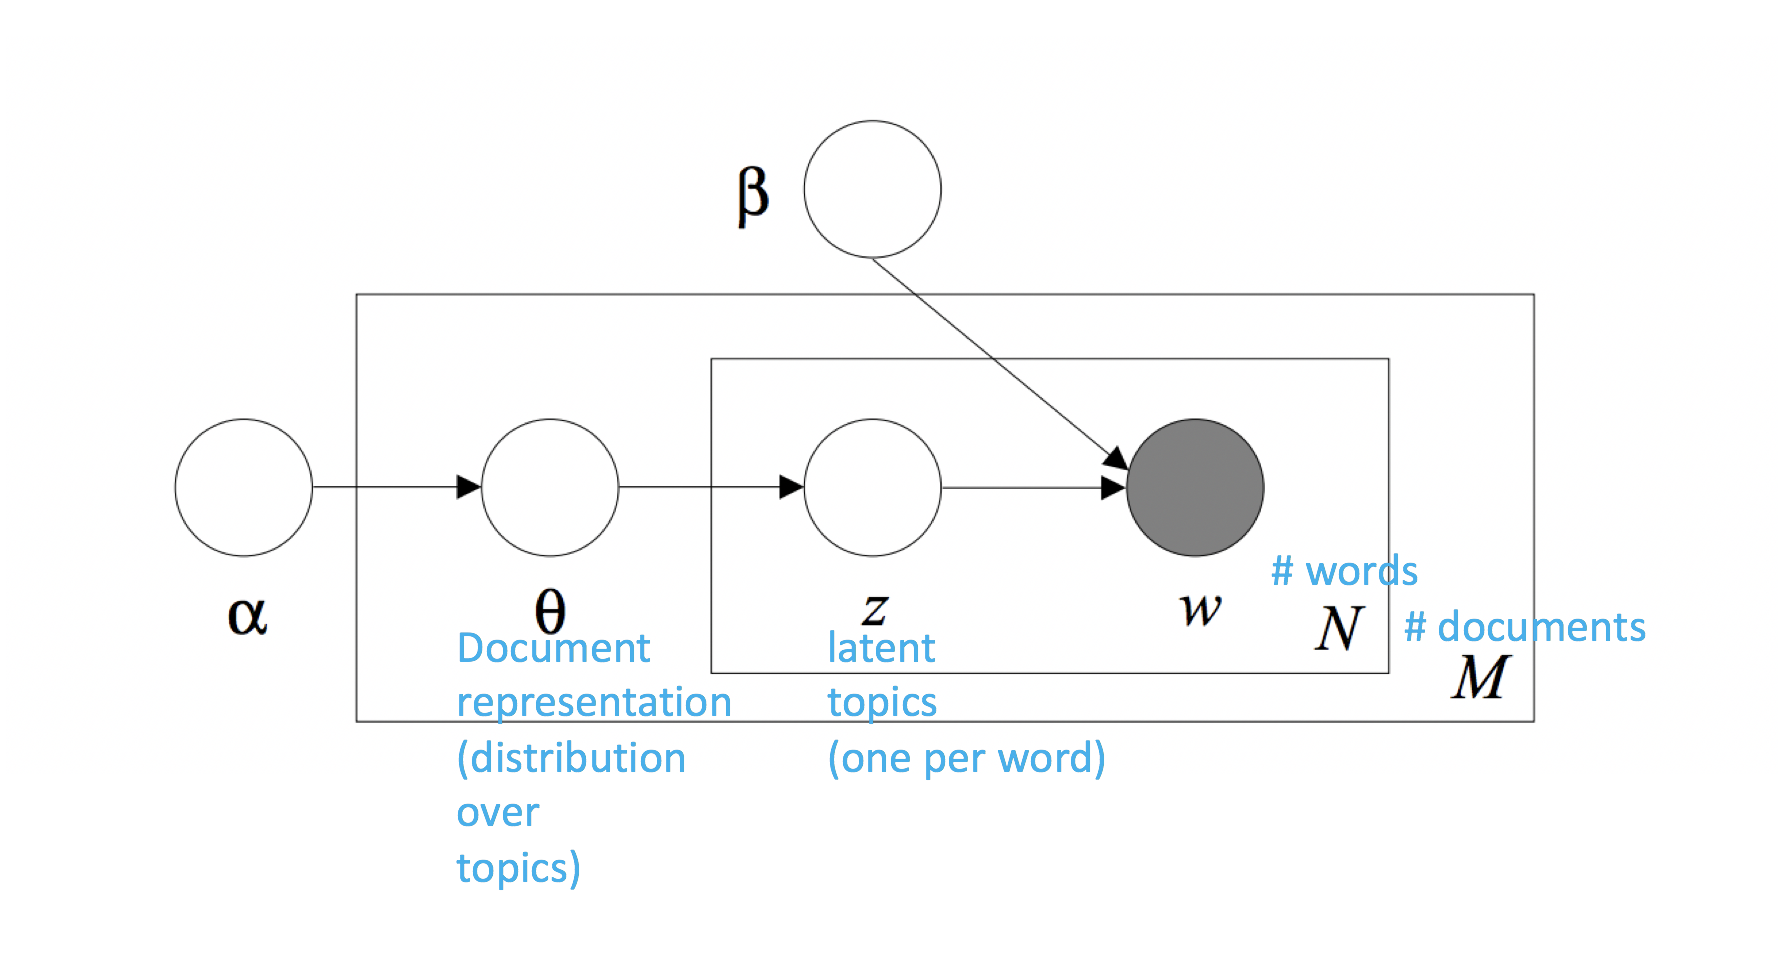
\includegraphics[width=\textwidth]{images/lda_generative.png}
%	\end{figure}
%
%\end{frame}
%
%%%%%%
%
%\begin{frame}{Generative process} 
%
%For each document $\+w=(\+w_1, \hdots, \+w_n)$ in a corpus, the generative model is   
%
%\vfill
%
%\begin{itemize}
%\item Choose a topic distribution for the document $\+\theta \sim \text{Dirichlet}_K (\+\alpha)$
%\item For each word $\+w_n$:
%
%	\begin{itemize}
%	\item Choose a topic  $\+z_n \sim \text{Multinoulli}_K (\theta)$ 
%	\item Choose a word $\+w_n \sim \text{Multinoulli}_V (\+\beta_{\+z_n, \cdot})$
%	\end{itemize}
%\end{itemize}
%
%%Note in particular that (for now) we have assumed access to $\+\beta$. 
%
%\vfill \vfill \vfill
%
%\textbf{Remark.} Note that LDA is a ``bag-of-words" model; i.e. the probability of a word (or document) is invariant to word order.
%
%\end{frame}
%
%%%%%%%%%%%%%%%%%%%%%%%%%%%%%%%%%%%%%%%%%%%%
%%%%%%%%%%%%%%%%%%%%%%%%%%%%%%%%%%%%%%%%%%%%
%
%
%
%
%%%%%%%%%%%%%%%%%%%%%%%%%%%%%%%%%%%%%%%%%%%%
%%%%%%%%%%%%%%%%%%%%%%%%%%%%%%%%%%%%%%%%%%%%
%
%\begin{frame}{Joint distribution}
%
%The joint distribution for the generative process is given by 
%
%\begin{equation}
%p(\+z, \+\theta, \+w \cond \+\alpha, \+\beta)  = \explainterm{Dirichlet}{p(\+\theta \cond \+\alpha)} \; \ds\prod_{n=1}^N \explainterm{Multinoulli}{p(\+z_n \cond \+\theta)} \; \explainterm{Multinoulli}{p(\+w_n \cond \+z_n, \+\beta)}
%\label{lda_joint}
%\end{equation}
%
%
%\begin{definition}{($[\cdot]$)}\label{brackets_op}
%We define the operator  $[\cdot] : OneHot(K) \to \set{1,...,K}$ as that which takes a one-hot encoded vector and returns the (unique) index which is non-zero.
%\end{definition} 
%
%Using Definition \ref{brackets_op}, we can specify the functional forms for the multinoulli log likelihoods as
%
%\begin{align}
%\log p(\+z_n \cond \+\theta) &= \log \+\theta_{[z_n]} \label{lda_log_like_latent} \\
%\log p(\+w_n \cond \+z_n, \+\beta) &=  \log \+\beta_{[\+z_n], [\+w_n]} \label{lda_log_like_observed}
%\end{align}
%
%
%\end{frame}
%
%
%%%%%%%%%%%%%%%%%%%%%%%%%%%%%%%%%%%%%%%%%%%%
%%%%%%%%%%%%%%%%%%%%%%%%%%%%%%%%%%%%%%%%%%%%
%
%\begin{frame}{Variational distribution}
%
%We approximate the posterior $p(\+\theta \cond \+z, \+w)$
%using mean field variational inference  \eqref{mean_field}. In particular, we assume that the variational family $\Q$ has a density which factorizes as
%
%\begin{align} 
%q &= q_\+\delta (\+\theta) \; q_\+\tau (\+z) \nonumber \\
%&=  \explaintermbrace{Dirichlet}{q_\+\delta (\+\theta)}  \; \ds\prod_{n=1}^N \; \explaintermbrace{Multinoulli}{q_{\+\tau_n} (\+z_n)} \label{mean_field_lda}
%\end{align}
%
%\end{frame}
%
%
%\begin{frame}{Update equations} 
%
%\metroset{block=fill}
%\begin{block}{LDA coordinate ascent update equations}
%\begin{align} 
%\explainterm{var. multinoulli (topics-for-word)}{\tau_{n,k}} &\propto  \bigg( \Psi(\delta_k) - \Psi (\ds\sum_j \delta_j) \bigg) \;\;  \beta_{k, [w_n]} 
% \label{multinomial_update} \\
% &=  \explainterm{var. "prior" \; over \; topics}{\exp \bigg\{ \biggE{q_\delta(\theta)}{\log \+\theta_i} \bigg\} } \;\; \explainterm{likelihood}{\beta_{k, [w_n]}}  \nonumber \\
%\explainterm{var. dirichlet (documents)}{\delta_k} &= \explainterm{prior counts}{\alpha_k} + \ds\sum_{n=1}^N \;\; \explainterm{var. prob of topics}{\tau_{n,k}} \label{dirichlet_update}
%\end{align}
%
%where $\Psi(\cdot)$ is the first derivative of the $\log \Gamma$ function. 
%\end{block}
%
%
%\begin{itemize}
%\item Derivable via VBEM (see notes). 
%\item Could also fit $\alpha, \beta$ to data via VEM; i.e. VEM does "empirical Bayes" for you.  
%\item Characteristic form: latent variable update depends on the data, global parameter update depends on the latent variable
%
%\end{itemize}
%
% 
%\end{frame}
%
%
%\begin{frame}{The role of analytical computations}
%
%The varational multinomial update crucially hinges on facts about the exponential family.  
%
%In particular, the meat of the proof of the variational multinomial update depends crucially on the fact that the Dirichlet of a single probability component is given by
%\begin{equation} \label{dirichlet_expect_prob_component}
% \biggE{q_\delta(\theta)}{\log \+\theta_i} =    \Psi(\delta_{i}) - \Psi (\ds\sum_k \delta_k) 
%\end{equation}
%where $\Psi(\cdot)$ is the first derivative of the $\log \Gamma$ function. 
%
%This fact is justified via facts about the exponential family (such as that the derivative of the log normalization factor with respect to the natural parameter is equal to the sufficient statistic). 
%
%\end{frame}
%
%
%%%%%%%%%%%%%%%%%%%%%%%%%%%%%%%%%%%%%%%%%%%%
%\begin{frame}{Summary}
%
%
%\begin{enumerate}
%\item We can derive \tiny (see notes) \normalsize the LDA update equations from the VBEM algorithm, so that we have  
%\[ \text{MF-CAVI} \rightarrow \text{VBEM} \rightarrow \text{LDA} \]
%and LDA instantiates the big picture.
%
%\item We have highlighted the potential obstacles for deriving VI updates via classical approaches.  This will foreshadow and motivate the development of black-box VI.
%\end{enumerate}
%%Also although old + simple, it HAS been cited 28,000 times, so nice to know about. 
%
%\end{frame}


%\section{Summary}
%\begin{frame}{Evaluation of CAVI}
%
%CAVI uses deterministic optimization methods, and thereby requires analytical expansions of the expectations. 
%
%\vfill
%
%\redx This can require expert analysis, in terms of setting up the model, carefully choosing the variational family, and carrying out the integrals.  Moreover, expert analysis is required each time the model changes.%\footnotesize Modern approaches, labeled \textit{generic variational inference} (\texttt{generic VI}) or \textit{black-box variational inference} (\bbvi) attempt to construct inference procedures that are invariant to choice of probability model, and therefore require limited or no expert analysis.  \normalsize
% 
%\vfill
%
%\greencheck  However, CAVI is still used in state-of-the-art models for efficient subroutines in black box models. %\footnotesize Indeed, exploiting efficient subroutines is a major theme in the  contemporary machine learning literature, which is exploring how to combine the complementary benefits of probabilistic graphical models and neural networks. E.g. see structured variational autoencoder (SVAE). 
%
%\end{frame}


\section{Automatic Differentiation Variational Inference (ADVI)}

\begin{frame}[fragile]{Coordinate ascent, and its discontents}


	\metroset{block=fill}
	\begin{block}{The ELBO (Evidence Lower Bound): Parametric View} 
			\begin{equation*}
			L(\lambda) = \E_{q_\lambda(z)} \bigg[ \log p(x,z) - \log q(z) \bigg]
			\end{equation*}
	
	\end{block}
	
\pause 
%		
		Traditionally, we optimize via coordinate-ascent (CAVI). 
			\begin{equation*}
		\widehat{\lambda}_{t+1} = \widehat{\lambda}_t + \rho_t \nabla L( \widehat{\lambda_t})
			\end{equation*}

\pause 
	\begin{alertblock}{Problem: Each model's VI algorithm is\only<3>\footnote{if it exists} a snowflake.} 
		\begin{itemize}
			\item Requires \textit{model-specific} computations %"a new paper for every model" exploiting model-specific facts, e.g. LDA.   
			\item Must pick a good $q$.  			
			%\item May be intractable. 
		\end{itemize}
	\end{alertblock}
      
\end{frame}

\begin{frame}{Differentiable Probability Models}

\metroset{block=fill}

\textsc{Goal:} Approximate the posterior $p(\+\theta \cond \+x) \propto p(\+x \cond \+\theta) p(\+\theta)$

\vspace{.05in}
\begin{block}{The class of probability models that ADVI supports}

	\vspace{.1in}
	\begin{minipage}[t][.33\textheight]{\textwidth}
		
	\begin{itemize}
	\item Dataset $\+x=x_{1:N}$ where each $x_n$ is a realization of a discrete or continuous random variable 
	\item Latent variables $\+\theta$ are continuous 
	\item $\nabla_\theta \log p(\+x, \+\theta)$ exists within the support of the prior 
	\[\Theta := \text{supp}(p(\+\theta)) = \{  \+\theta \cond \+\theta \in \R^K \text{ and } p(\+\theta) > 0 \} \subseteq \R^K \]
	\end{itemize}

	\end{minipage}
\end{block}	

\vspace{.05in}
	\begin{columns}[t]
	\column{.45\textwidth}
	\textsc{Includes}  \\
	\textit{Generalized linear models} \\ %\small (e.g., linear, logistic, Poisson) \normalsize 
	\textit{Mixture models} \\
	\textit{Topic models} \\  %\small (e.g., latent Dirichlet allocation)\\
	\textit{Linear dynamic systems} \\
	\textit{Gaussian process models} \\
	\textit{Deep exponential families} \\
	\column{.45\textwidth}
	\textsc{Excludes} \\
	\textit{Ising model} \\
	\textit{Sigmoid belief networks} \\
	\textit{Bayesian nonparametric models}
	\vfill
	
	\end{columns}
	

\end{frame}



%\begin{frame}{Review: Change of Variables} 
%\metroset{block=fill}
%\begin{block}{Change of variables}
%
%Under some assumptions on $f$ and $T$, 
%%\[ \ds\int_{\Theta} p(x,\theta) \; d\theta = \ds\int_{\R^K} p\big(x, T(\theta)\big) \logabsdet{J_T (\theta)} \; d \theta \] 
%
%\[ \ds\int_{\Theta} f(\theta) \; d\theta = \ds\int_{\R^K} f\big(T(\theta)\big) \absdet{J_T (\theta)} \; d \theta \] 
%
%\footnotesize
%The intuition runs as follows:
%
%\begin{itemize}
%\item \textit{(Volume warping)} Let $A \in \R^{n \times n}, S \subset \R^n$.  Then $m(AS) = \absdet{A} m(s)$.    (To see this, recall the SVD $A=U \Sigma V^T$ and $\absdet{A} = \det{\Sigma}$.) 
%\item \textit{(Taylor expansion)} Let $\theta$ be a small set, $\theta_i \in \theta$. Then
%\begin{align*}
%T(\theta) & \approx T(\theta_i) + J_T(\theta_i) (\theta - \theta_i)\\
%\implies m(T(\theta)) & \approx \absdet{J_T(\theta_i)} m(\theta) 
%\end{align*}
%\end{itemize}
%\end{block}
%
%\end{frame}

\begin{frame}{Step 1: Transforming to unbounded support}
\small

%Real-valued parameters support 1) model-independent variational approximations, 2) gradient descent without leaving $\Theta$, 3) the \textit{reparameterization trick.}

We define a differentiable bijection to give the parameters unbounded support.
\begin{align*}
T : \Theta & \to \R^K \\
	\theta & \mapsto \zeta
\end{align*}

We use \textit{change of variables} to express the joint density in the new space. \normalsize

%	\[ \redbox{t1}{p(\+x,\+\zeta)}  = \underset{\blue{original \; space}}{\bluebox{t2}{ 
%	$p\big(\+x, T^{-1}(\+\zeta)\big)  \logabsdet{J_{T^{-1}} (\+\zeta)}$
%	}}\]
	\[ \labeledgreenbox{new \; space}{p(\+x,\+\zeta)}  = \labeledbluebox{transformed \; original \; space}{$p\big(\+x, T^{-1}(\+\zeta)\big)  \absdet{J_{T^{-1}} (\+\zeta)}$}\]
	
So in the new space, the ELBO becomes 
\[ \mathcal{L}(\+\lambda) = \E_{q(\+\zeta; \+\lambda)}  \bigg[ 
	\bluebox{
	$\log p \big(\+x, T^{-1}(\+\zeta)\big) + \logabsdet{J_{T^{-1}} (\+\zeta)}$
	} 
\bigg]  + \mathbb{H} [q(\+\zeta ; \+\lambda )] \] 

\pause
\vspace{.1in}
\begin{columns}
\column{.55\textwidth}
\small 
\greencheck Model-independent variational factors. \\
\column{.44\textwidth}
\small
\redx Cannot compute the gradient of the cost function \pause {\tiny (Think: Why can't we just approximate the term by sampling?)} \\
\end{columns}	
\end{frame}
%SAY: The problem is, we still can't optimize this function, because the expectation is, in general, intractable. 


\begin{frame}{Step 2: The reparameterization trick}
	
\textbf{Example}: We can \textit{re-parameterize} the Gaussian $\+\zeta \sim \mathcal{N}(\+\mu, \+\Sigma)$, such that its dependence on the original parameter $\+\lambda = (\+\mu, \+\Sigma)$ is transferred to a (deterministic) standardization function, $S_\+\lambda$ 
%\footnote{assumed continuously differentiable and invertible}, $S_\+\lambda$ 

\begin{itemize}
\item Factorize $\+\Sigma=\+L\+L^T$. 
\item The standardized random variable is 
\[ \+\epsilon := S_{\+\lambda} (\+\zeta) = \+L^{-1} (\+\zeta - \+\mu), \quad \text{ where } \+\epsilon \sim \mathcal{N}(\+0, \+I)\]  
\item The unstandardized random variable can be recovered via
\[ \+\zeta = S_\+\lambda^{-1}(\+\epsilon)\]
\end{itemize}

\metroset{block=fill}
\begin{block}{\textsc{ADVI ELBO}}
\scriptsize
\[ \mathcal{L}(\+\lambda) = \E_{\norm (\+\epsilon; \+0, \+I)}  \bigg[ 
	\log p \bigg( \+x, T^{-1} \big( S^{-1}_{\+\lambda} (\+\epsilon) \big) \bigg) + \logabsdet{J_{T^{-1}} \big( S^{-1}_\+\lambda (\+\epsilon) \big)}  \bigg]  + \mathbb{H} [q(\+\zeta ; \+\lambda )] \] 
\normalsize
\end{block}

\pause
\vspace{.1in}
\begin{columns}
\column{.55\textwidth}
\small 
\greencheck Model-independent variational factors. \\
\column{.44\textwidth}
\small
\greencheck Can estimate the gradient of the expectation.\\
\end{columns}
	 	
	 	
\end{frame}


%%NOTES SLIDE 
%\begin{frame}[standout]
% 	Notes!
%\end{frame}


%QUESTIONS SLIDE 
\begin{frame}[standout]
  Questions?
\end{frame}



%%%%%%%%%%%%%
% Slide Graveyard
%%%%%%%%%%%



\end{document}








\subsection{Update equations} \label{lda_update_equations}

The coordinate ascent update equations are given by 
\begin{align} 
\tau_{n,k} &= \propto \beta_{k, [w_n]} \bigg( \Psi(\delta_k) - \Psi (\ds\sum_j \delta_j) \bigg) \label{multinomial_update} \\
\delta_k &= \alpha_k + \ds\sum_{n=1}^N \tau_{n,k} \label{dirichlet_update}
\end{align}
where $\Psi(\cdot)$ is the first derivative of the $\log \Gamma$ function. 

For a proof using the VBEM Algorithm, see Appendix \ref{lda_updates_derivation}.






